\chapter{Appendix}

\section{Additional Results and complete tables relative to Random Forest}\label{sec:RFAdditional}

Here are the tables with all of the features from random forest. There is no real utility in providing them for all possible feature combination, hence only the importances for all features will be given.
This will be done for both labels used, i.e. Death and ICU Admission. 

\centering
\begin{longtable}{|lr|}
\toprule
Feature Name &  Importance estimated by Random Forest \\
\midrule
Age (years)                                        &        0.056516 \\
CURB65                                             &        0.023775 \\
Intensity histogram quartile coefficient of dis... &        0.021053 \\
Discretised interquartile range                    &        0.017892 \\
Ground-glass                                       &        0.015137 \\
Dependence count entropy                           &        0.014432 \\
Intensity-based interquartile range                &        0.014269 \\
Small zone emphasis                                &        0.014180 \\
Zone size entropy                                  &        0.013493 \\
Normalised zone size non-uniformity                &        0.013321 \\
Skewness                                           &        0.013009 \\
Dependence count energy                            &        0.012736 \\
Information correlation 1                          &        0.011409 \\
Information correlation 2                          &        0.011391 \\
Intensity-based median absolute deviation          &        0.011173 \\
Quartile coefficient of dispersion                 &        0.010367 \\
Respiratory Rate                                   &        0.010176 \\
Entropy                                            &        0.009969 \\
Intensity histogram median absolute deviation      &        0.009406 \\
Run entropy                                        &        0.009264 \\
Volume density - enclosing ellipsoid               &        0.009191 \\
Intensity histogram robust mean absolute deviation &        0.009046 \\
Uniformity                                         &        0.008612 \\
Discretised intensity skewness                     &        0.008386 \\
Intensity-based robust mean absolute deviation     &        0.008134 \\
Maximum histogram gradient intensity               &        0.007806 \\
Grey level variance (GLDZM)                        &        0.007664 \\
Intensity-based mean absolute deviation            &        0.007580 \\
Normalised grey level non-uniformity (NGLDM)       &        0.007455 \\
Fat.surface                                        &        0.007220 \\
Febbre                                             &        0.007157 \\
Sum entropy                                        &        0.006892 \\
Local intensity peak                               &        0.006887 \\
Minor axis length (cm)                             &        0.006875 \\
Area density - enclosing ellipsoid                 &        0.006777 \\
Grey level variance (GLSZM)                        &        0.006726 \\
Angular second moment                              &        0.006453 \\
Cluster shade                                      &        0.006377 \\
XRayTubeCurrent                                    &        0.006247 \\
Max value                                          &        0.006077 \\
Zone distance non-uniformity                       &        0.005951 \\
Normalised zone distance non-uniformity            &        0.005922 \\
Small distance emphasis                            &        0.005790 \\
Cluster prominence                                 &        0.005772 \\
RECIST (cm)                                        &        0.005728 \\
Large distance high grey level emphasis            &        0.005609 \\
Normalised grey level non-uniformity (GLRLM)       &        0.005479 \\
Low dependence emphasis                            &        0.005422 \\
Small distance low grey level emphasis             &        0.005405 \\
Normalised grey level non-uniformity (GLSZM)       &        0.005318 \\
Grey level non-uniformity (NGLDM)                  &        0.005307 \\
Volume density - convex hull                       &        0.005301 \\
Volume at intensity fraction 90\%                   &        0.005267 \\
Large distance emphasis                            &        0.005247 \\
Normalised homogeneity                             &        0.005180 \\
Dependence count non-uniformity                    &        0.005174 \\
Small zone low grey level emphasis                 &        0.005110 \\
Number of grey levels                              &        0.005006 \\
Area density - convex hull                         &        0.004984 \\
Low grey level zone emphasis.1                     &        0.004983 \\
10th intensity percentile                          &        0.004967 \\
Intensity histogram mean absolute deviation        &        0.004965 \\
Intensity median value                             &        0.004960 \\
Discretised intensity kurtosis                     &        0.004954 \\
Energy                                             &        0.004950 \\
High dependence low grey level emphasis            &        0.004895 \\
Integrated intensity                               &        0.004888 \\
Small distance high grey level emphasis            &        0.004863 \\
Normalised inverse difference                      &        0.004814 \\
Zone distance entropy                              &        0.004801 \\
Normalised grey level non-uniformity (GLDZM)       &        0.004749 \\
Difference average                                 &        0.004743 \\
Thresholded area intensity peak (50\%)              &        0.004735 \\
Centre of mass shift (cm)                          &        0.004683 \\
Minimum histogram gradient                         &        0.004634 \\
Number of voxels                                   &        0.004592 \\
Low grey level zone emphasis                       &        0.004470 \\
Area density - oriented bounding box               &        0.004465 \\
Volume density - aligned bounding box              &        0.004453 \\
High dependence emphasis                           &        0.004453 \\
Intensity-based coefficient of variation           &        0.004442 \\
Thresholded area intensity peak (75\%)              &        0.004426 \\
Discretised intensity uniformity                   &        0.004342 \\
Low grey level count emphasis                      &        0.004310 \\
Grey level non-uniformity (GLDZM)                  &        0.004261 \\
Contrast (GLCM)                                    &        0.004247 \\
Difference entropy                                 &        0.004174 \\
Kurtosis                                           &        0.004151 \\
Grey level non-uniformity (GLRLM)                  &        0.004114 \\
Number of compartments (GMM)                       &        0.004110 \\
Intensity-based energy                             &        0.004093 \\
Small zone high grey level emphasis                &        0.004086 \\
Least axis length (cm)                             &        0.004086 \\
Intensity histogram mode                           &        0.004073 \\
Volume density - oriented bounding box             &        0.004064 \\
Inverse variance                                   &        0.004055 \\
Difference variance                                &        0.004024 \\
Surface to volume ratio                            &        0.003966 \\
Run length variance                                &        0.003913 \\
Variance                                           &        0.003910 \\
Correlation                                        &        0.003908 \\
Muscle.surface                                     &        0.003907 \\
High grey level zone emphasis                      &        0.003879 \\
Number of voxels of positive value                 &        0.003857 \\
Inverse elongation                                 &        0.003853 \\
Cluster tendency                                   &        0.003820 \\
Intensity range                                    &        0.003804 \\
Normalised run length non-uniformity               &        0.003799 \\
Large zone high grey level emphasis                &        0.003776 \\
Long run low grey level emphasis                   &        0.003766 \\
Area density - aligned bounding box                &        0.003687 \\
Zone percentage (GLDZM)                            &        0.003660 \\
Asphericity                                        &        0.003657 \\
Grey level variance (NGLDM)                        &        0.003643 \\
Intensity at volume fraction 90\%                   &        0.003617 \\
Volume at intensity fraction 10\%                   &        0.003610 \\
Major axis length (cm)                             &        0.003604 \\
Low dependence low grey level emphasis             &        0.003570 \\
Run length non-uniformity                          &        0.003548 \\
Strength                                           &        0.003459 \\
Long run high grey level emphasis                  &        0.003433 \\
Mean discretised intensity                         &        0.003413 \\
Low dependence high grey level emphasis            &        0.003409 \\
Dissimilarity                                      &        0.003395 \\
High grey level count emphasis                     &        0.003394 \\
SliceThickness                                     &        0.003389 \\
Grey level non-uniformity (GLSZM)                  &        0.003381 \\
Volume fraction difference between intensity fr... &        0.003381 \\
Grey level variance (GLRLM)                        &        0.003369 \\
Short run low grey level emphasis                  &        0.003347 \\
Maximum histogram gradient                         &        0.003338 \\
High dependence high grey level emphasis           &        0.003321 \\
Compactness 2                                      &        0.003317 \\
Long run emphasis                                  &        0.003316 \\
Autocorrelation                                    &        0.003261 \\
Joint maximum                                      &        0.003254 \\
Global intensity peak                              &        0.003237 \\
Sum average                                        &        0.003233 \\
Low grey level run emphasis                        &        0.003187 \\
Dependence count variance                          &        0.003182 \\
Intensity at volume fraction 10\%                   &        0.003128 \\
Large distance low grey level emphasis             &        0.003125 \\
Zone percentage (GLSZM)                            &        0.003088 \\
Intensity fraction difference between volume fr... &        0.003034 \\
Zone distance variance                             &        0.002949 \\
Maximum 3D diameter (cm)                           &        0.002940 \\
Normalized dependence count non-uniformity         &        0.002937 \\
Inverse difference                                 &        0.002912 \\
Intensity histogram coefficient of variation       &        0.002872 \\
Coarseness                                         &        0.002836 \\
Run percentage                                     &        0.002805 \\
Flatness                                           &        0.002788 \\
Standard deviation                                 &        0.002760 \\
Joint variance                                     &        0.002714 \\
Busyness                                           &        0.002711 \\
Intensity mean value                               &        0.002706 \\
Homogeneity                                        &        0.002698 \\
Large zone low grey level emphasis                 &        0.002665 \\
Joint average                                      &        0.002614 \\
KVP                                                &        0.002597 \\
90th discretised intensity percentile              &        0.002525 \\
90th intensity percentile                          &        0.002523 \\
Contrast (NGTDM)                                   &        0.002511 \\
Joint Entropy                                      &        0.002488 \\
Spherical disproportion                            &        0.002455 \\
Sphericity                                         &        0.002423 \\
Discretised intensity standard deviation           &        0.002377 \\
Compactness 1                                      &        0.002372 \\
Crazy Paving                                       &        0.002324 \\
Area under the IVH curve                           &        0.002259 \\
High grey level run emphasis                       &        0.002258 \\
Complexity                                         &        0.002223 \\
Short run emphasis                                 &        0.002206 \\
Discretised intensity variance                     &        0.002196 \\
Large zone emphasis                                &        0.002158 \\
Short run high grey level emphasis                 &        0.002158 \\
High grey level zone emphasis.1                    &        0.002006 \\
Median discretised intensity                       &        0.001935 \\
Min value                                          &        0.001904 \\
Quadratic mean                                     &        0.001870 \\
Obesity                                            &        0.001766 \\
Discretised intensity entropy                      &        0.001680 \\
Sex\_bin                                            &        0.001662 \\
Minimum histogram gradient intensity               &        0.001547 \\
Sum variance                                       &        0.001496 \\
Lung consolidation                                 &        0.000751 \\
Bilateral Involvement                              &        0.000694 \\
History of smoking                                 &        0.000513 \\
Hypertension                                       &        0.000493 \\
Discretised max value                              &        0.000000 \\
Discretised min value                              &        0.000000 \\
Discretized intensity range                        &        0.000000 \\
Dependence count percentage                        &        0.000000 \\
Number of grey levels after quantization           &        0.000000 \\
HRCT performed                                     &        0.000000 \\
\bottomrule
\caption{Importances determined by RandomForest predicting death using all available features. The values are in descending order.} % needs to go inside longtable environment
\label{tab:RFimpoAllDeath}
\end{longtable}

\centering
\begin{longtable}{|lr|}
\toprule
{} &  RF\_importances \\
\midrule
Age (years)                                        &        0.043174 \\
Sex\_bin                                            &        0.020316 \\
Fat.surface                                        &        0.017942 \\
Dependence count entropy                           &        0.017538 \\
Dependence count energy                            &        0.015580 \\
Respiratory Rate                                   &        0.012740 \\
Intensity histogram quartile coefficient of dis... &        0.012675 \\
Flatness                                           &        0.012201 \\
Discretised interquartile range                    &        0.012029 \\
Small zone high grey level emphasis                &        0.011807 \\
Run entropy                                        &        0.010264 \\
Intensity histogram median absolute deviation      &        0.010097 \\
Least axis length (cm)                             &        0.009921 \\
Muscle.surface                                     &        0.009778 \\
Dependence count variance                          &        0.009557 \\
Angular second moment                              &        0.009544 \\
Quartile coefficient of dispersion                 &        0.009437 \\
Large distance high grey level emphasis            &        0.009423 \\
Joint Entropy                                      &        0.009381 \\
Low dependence high grey level emphasis            &        0.009338 \\
SliceThickness                                     &        0.009026 \\
Inverse elongation                                 &        0.008748 \\
Intensity-based interquartile range                &        0.008110 \\
Information correlation 2                          &        0.008001 \\
Run length variance                                &        0.007324 \\
Dependence count non-uniformity                    &        0.007150 \\
Energy                                             &        0.006935 \\
Global intensity peak                              &        0.006818 \\
Normalized dependence count non-uniformity         &        0.006794 \\
RECIST (cm)                                        &        0.006689 \\
Maximum 3D diameter (cm)                           &        0.006610 \\
Lung consolidation                                 &        0.006506 \\
Centre of mass shift (cm)                          &        0.006447 \\
Max value                                          &        0.006395 \\
Information correlation 1                          &        0.006361 \\
Compactness 1                                      &        0.006337 \\
Run percentage                                     &        0.006314 \\
Long run emphasis                                  &        0.006191 \\
Short run emphasis                                 &        0.006061 \\
Zone distance non-uniformity                       &        0.006042 \\
Sphericity                                         &        0.005936 \\
Normalised run length non-uniformity               &        0.005929 \\
Autocorrelation                                    &        0.005853 \\
High grey level zone emphasis.1                    &        0.005797 \\
Volume density - convex hull                       &        0.005778 \\
Integrated intensity                               &        0.005719 \\
Volume density - oriented bounding box             &        0.005678 \\
Intensity histogram robust mean absolute deviation &        0.005671 \\
Volume at intensity fraction 90\%                   &        0.005601 \\
Normalised homogeneity                             &        0.005591 \\
Inverse difference                                 &        0.005562 \\
Local intensity peak                               &        0.005533 \\
Area density - oriented bounding box               &        0.005528 \\
Inverse variance                                   &        0.005505 \\
Intensity-based energy                             &        0.005463 \\
Crazy Paving                                       &        0.005460 \\
Sum entropy                                        &        0.005449 \\
Homogeneity                                        &        0.005447 \\
Small distance low grey level emphasis             &        0.005413 \\
Asphericity                                        &        0.005396 \\
Thresholded area intensity peak (50\%)              &        0.005375 \\
Minimum histogram gradient                         &        0.005369 \\
High dependence high grey level emphasis           &        0.005369 \\
Contrast (GLCM)                                    &        0.005365 \\
Zone distance variance                             &        0.005334 \\
Surface to volume ratio                            &        0.005209 \\
Volume density - aligned bounding box              &        0.005162 \\
Spherical disproportion                            &        0.005159 \\
Sum average                                        &        0.005132 \\
High dependence low grey level emphasis            &        0.005112 \\
Area density - convex hull                         &        0.005111 \\
Grey level variance (GLDZM)                        &        0.005107 \\
Compactness 2                                      &        0.004996 \\
Number of voxels of positive value                 &        0.004984 \\
Discretised intensity uniformity                   &        0.004979 \\
KVP                                                &        0.004974 \\
Cluster shade                                      &        0.004964 \\
Thresholded area intensity peak (75\%)              &        0.004958 \\
Grey level non-uniformity (GLDZM)                  &        0.004918 \\
Normalised zone distance non-uniformity            &        0.004912 \\
Number of grey levels                              &        0.004905 \\
Grey level non-uniformity (NGLDM)                  &        0.004786 \\
Dissimilarity                                      &        0.004767 \\
Large zone high grey level emphasis                &        0.004756 \\
Complexity                                         &        0.004710 \\
Cluster prominence                                 &        0.004679 \\
Low dependence low grey level emphasis             &        0.004673 \\
Area density - aligned bounding box                &        0.004666 \\
Long run high grey level emphasis                  &        0.004659 \\
Grey level variance (GLSZM)                        &        0.004627 \\
Normalised zone size non-uniformity                &        0.004610 \\
Strength                                           &        0.004605 \\
Normalised grey level non-uniformity (NGLDM)       &        0.004563 \\
Difference variance                                &        0.004546 \\
Correlation                                        &        0.004544 \\
CURB65                                             &        0.004524 \\
Normalised grey level non-uniformity (GLRLM)       &        0.004522 \\
Small zone emphasis                                &        0.004512 \\
Volume at intensity fraction 10\%                   &        0.004447 \\
Large distance emphasis                            &        0.004423 \\
Minor axis length (cm)                             &        0.004406 \\
Zone distance entropy                              &        0.004374 \\
XRayTubeCurrent                                    &        0.004373 \\
Area density - enclosing ellipsoid                 &        0.004333 \\
Small distance high grey level emphasis            &        0.004326 \\
Contrast (NGTDM)                                   &        0.004271 \\
Low dependence emphasis                            &        0.004255 \\
Short run high grey level emphasis                 &        0.004209 \\
Small zone low grey level emphasis                 &        0.004182 \\
Difference average                                 &        0.004180 \\
Intensity range                                    &        0.004178 \\
High grey level zone emphasis                      &        0.004157 \\
Intensity-based robust mean absolute deviation     &        0.004130 \\
Intensity histogram coefficient of variation       &        0.004124 \\
Difference entropy                                 &        0.004122 \\
Major axis length (cm)                             &        0.004113 \\
Volume fraction difference between intensity fr... &        0.004113 \\
Low grey level count emphasis                      &        0.004092 \\
Intensity median value                             &        0.004051 \\
Uniformity                                         &        0.004049 \\
Grey level non-uniformity (GLRLM)                  &        0.004033 \\
High grey level run emphasis                       &        0.004027 \\
Number of voxels                                   &        0.004015 \\
Joint variance                                     &        0.003956 \\
Run length non-uniformity                          &        0.003941 \\
Discretised intensity entropy                      &        0.003905 \\
Zone percentage (GLDZM)                            &        0.003893 \\
Large zone low grey level emphasis                 &        0.003886 \\
Sum variance                                       &        0.003878 \\
Low grey level zone emphasis                       &        0.003853 \\
Zone percentage (GLSZM)                            &        0.003821 \\
High grey level count emphasis                     &        0.003811 \\
Busyness                                           &        0.003795 \\
High dependence emphasis                           &        0.003757 \\
Grey level non-uniformity (GLSZM)                  &        0.003727 \\
Large distance low grey level emphasis             &        0.003638 \\
Volume density - enclosing ellipsoid               &        0.003633 \\
Zone size entropy                                  &        0.003558 \\
Joint maximum                                      &        0.003558 \\
Discretised intensity skewness                     &        0.003552 \\
Skewness                                           &        0.003496 \\
Grey level variance (NGLDM)                        &        0.003480 \\
Area under the IVH curve                           &        0.003470 \\
Normalised grey level non-uniformity (GLDZM)       &        0.003468 \\
Intensity histogram mean absolute deviation        &        0.003431 \\
Normalised inverse difference                      &        0.003320 \\
Short run low grey level emphasis                  &        0.003299 \\
Mean discretised intensity                         &        0.003293 \\
Low grey level zone emphasis.1                     &        0.003285 \\
Discretised intensity kurtosis                     &        0.003275 \\
Small distance emphasis                            &        0.003148 \\
Joint average                                      &        0.003141 \\
Intensity-based median absolute deviation          &        0.003112 \\
90th discretised intensity percentile              &        0.003094 \\
Large zone emphasis                                &        0.003052 \\
90th intensity percentile                          &        0.003030 \\
10th intensity percentile                          &        0.003021 \\
Low grey level run emphasis                        &        0.002930 \\
Kurtosis                                           &        0.002860 \\
Cluster tendency                                   &        0.002743 \\
Intensity at volume fraction 10\%                   &        0.002725 \\
Grey level variance (GLRLM)                        &        0.002673 \\
Long run low grey level emphasis                   &        0.002640 \\
Intensity-based coefficient of variation           &        0.002634 \\
Min value                                          &        0.002620 \\
Intensity mean value                               &        0.002595 \\
Entropy                                            &        0.002562 \\
Normalised grey level non-uniformity (GLSZM)       &        0.002561 \\
Variance                                           &        0.002516 \\
Minimum histogram gradient intensity               &        0.002509 \\
Discretised intensity standard deviation           &        0.002474 \\
Maximum histogram gradient intensity               &        0.002467 \\
Standard deviation                                 &        0.002411 \\
Maximum histogram gradient                         &        0.002410 \\
Intensity at volume fraction 90\%                   &        0.002390 \\
Quadratic mean                                     &        0.002362 \\
Intensity fraction difference between volume fr... &        0.002215 \\
Intensity-based mean absolute deviation            &        0.002203 \\
Discretised intensity variance                     &        0.001964 \\
Intensity histogram mode                           &        0.001620 \\
Coarseness                                         &        0.001438 \\
Median discretised intensity                       &        0.001337 \\
Number of compartments (GMM)                       &        0.001055 \\
Obesity                                            &        0.000973 \\
History of smoking                                 &        0.000896 \\
Bilateral Involvement                              &        0.000893 \\
Ground-glass                                       &        0.000859 \\
Hypertension                                       &        0.000497 \\
Febbre                                             &        0.000358 \\
HRCT performed                                     &        0.000000 \\
Discretized intensity range                        &        0.000000 \\
Discretised min value                              &        0.000000 \\
Discretised max value                              &        0.000000 \\
Dependence count percentage                        &        0.000000 \\
Number of grey levels after quantization           &        0.000000 \\
\bottomrule
\caption{Importances determined by RandomForest predicting ICU Admission using all available features. The values are in descending order.} % needs to go inside longtable environment
\label{tab:RFimpoRad}
\end{longtable}

\section{Using Dimensionality reduction to further investigate the dataset}
For these analyses the data was always fed into a standard scaler before applying the technique of choice, furthermore a custom gravity score by classifying as 4 the dead individuals and then by assigning a progressive score form 1 to 3 by looking at the time of permanence was built as follows:

\begin{enumerate}
\item Gravity 1: Survived individuals with permanence from 0$^{th}$ percentile to 25$^{th}$ percentile
\item Gravity 2:Survived individuals with permanence from 25$^{th}$ percentile to 75$^{th}$ percentile
\item Gravity 3:Survived individuals with permanence from 75$^{th}$ percentile to 100$^{th}$ percentile
\item Gravity 4: Dead individuals without regard for permanence in the hospital
\end{enumerate}

\begin{figure}[htbp]
	\centering 
  		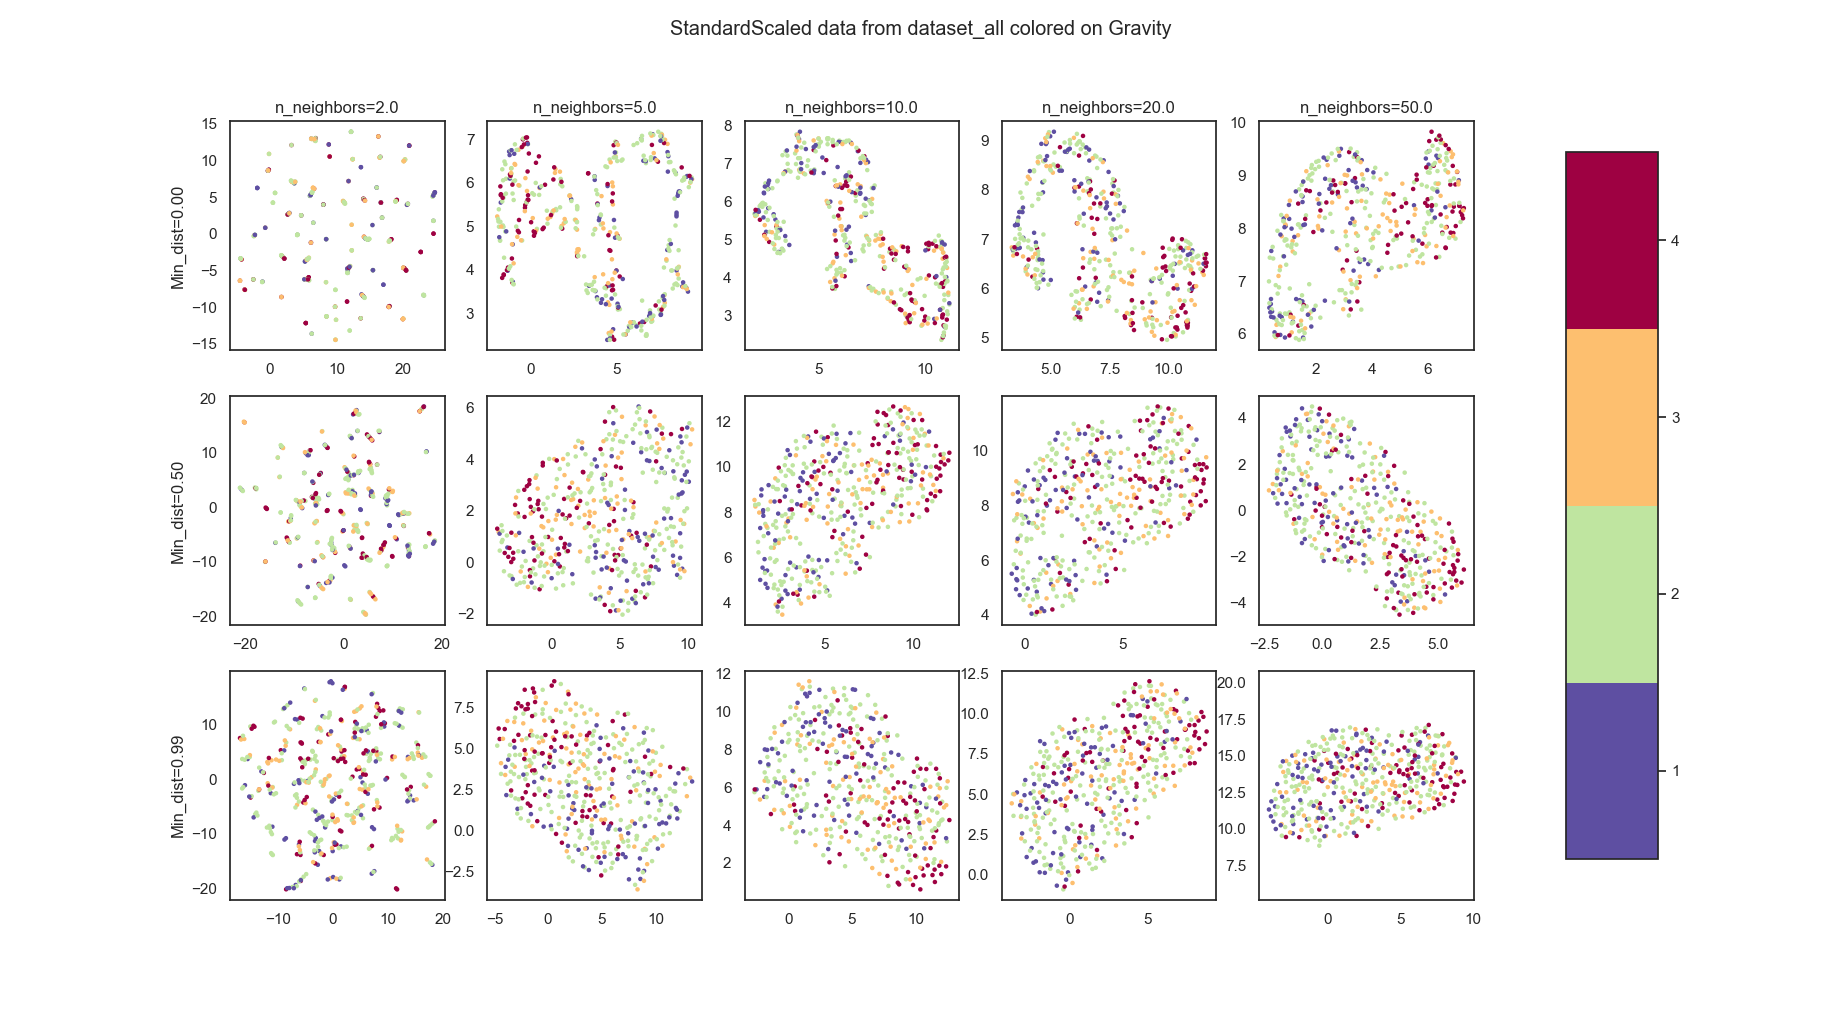
\includegraphics[width = \linewidth]{Scale_umap_gravityquantilies2575.png}
        \caption{Possible combination for umap hyperparameters "number of neighbours" and "minimum distance". Color coding is done with aforementioned gravity score and all the features, i.e. clinical radiomic and radiological, were used.  \label{fig:hyperparam_umap}}
\end{figure}


Also, before proceeding, the hyperparameter space for umap was explored since it's the method that allows the most control over rather intuitive parameters.
Changing the value of the minimum distance of points in the final space from 0 to 0.99 changes how the structure is projected, while changing the number of neighbours changes how much the local or global structure of the data influences the final projection.
 Some of the combinations of these parameters can be seen in Figure \ref{fig:hyperparam_umap}


\subsection{Explaining total variance using PCA}

Starting from PCA, the data was reduced to either two or three dimensions considering clinical and radiomic features, both separated and together.
In this first example there seems to be a kind of left leaning polarization of the dead individuals, however there are no clear separations in the data.

\begin{figure}[h!]
\centering
  		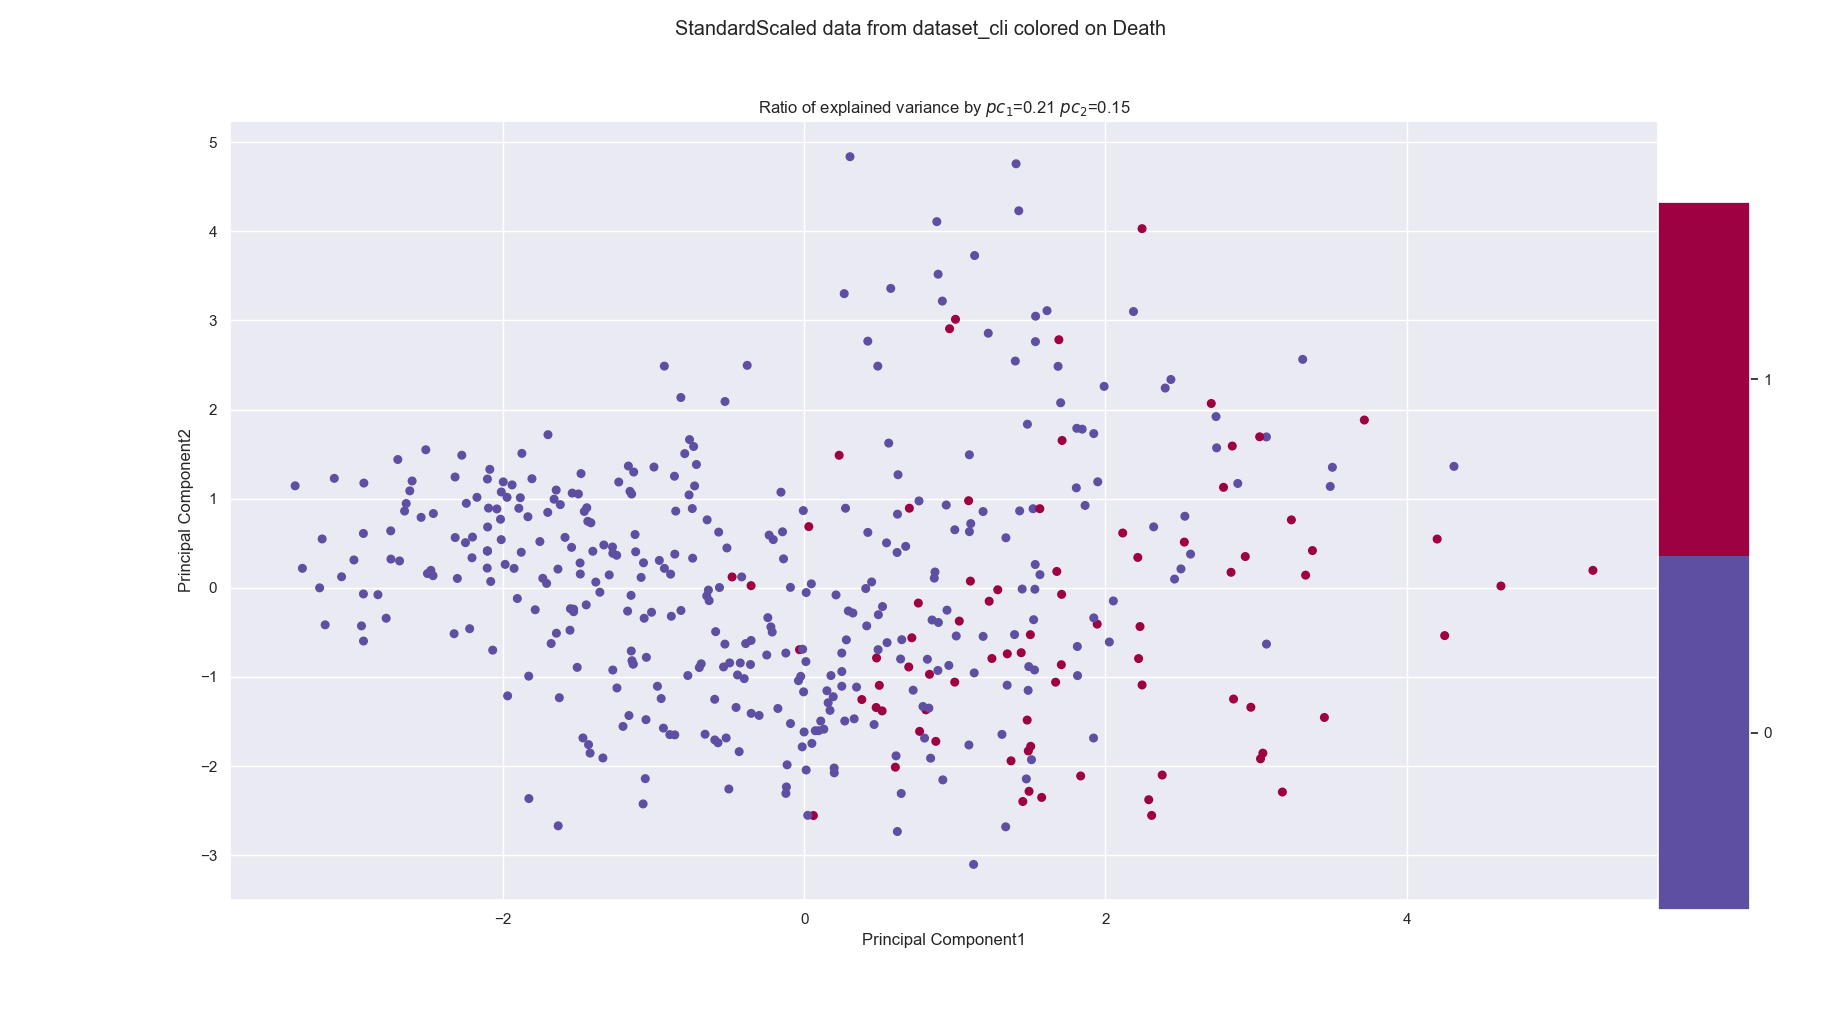
\includegraphics[width=\linewidth]{PCA2_Death.png}
        \caption{2-Principal Component on clinical features.  \label{fig:PCA2_death}}
\end{figure}

 Working on the clinical dataset it can also be noted that the first two components of the PCA explain only 36$\%$ of the total variance. This leads to the conclusion that changes in the data cannot be explained by a single, nor a few, features or linear combination thereof. The next approach was  using the first three principal components using various labels available, most relevant of which being ICU admission, Death and Gravity score.

\begin{figure}[h!]
  		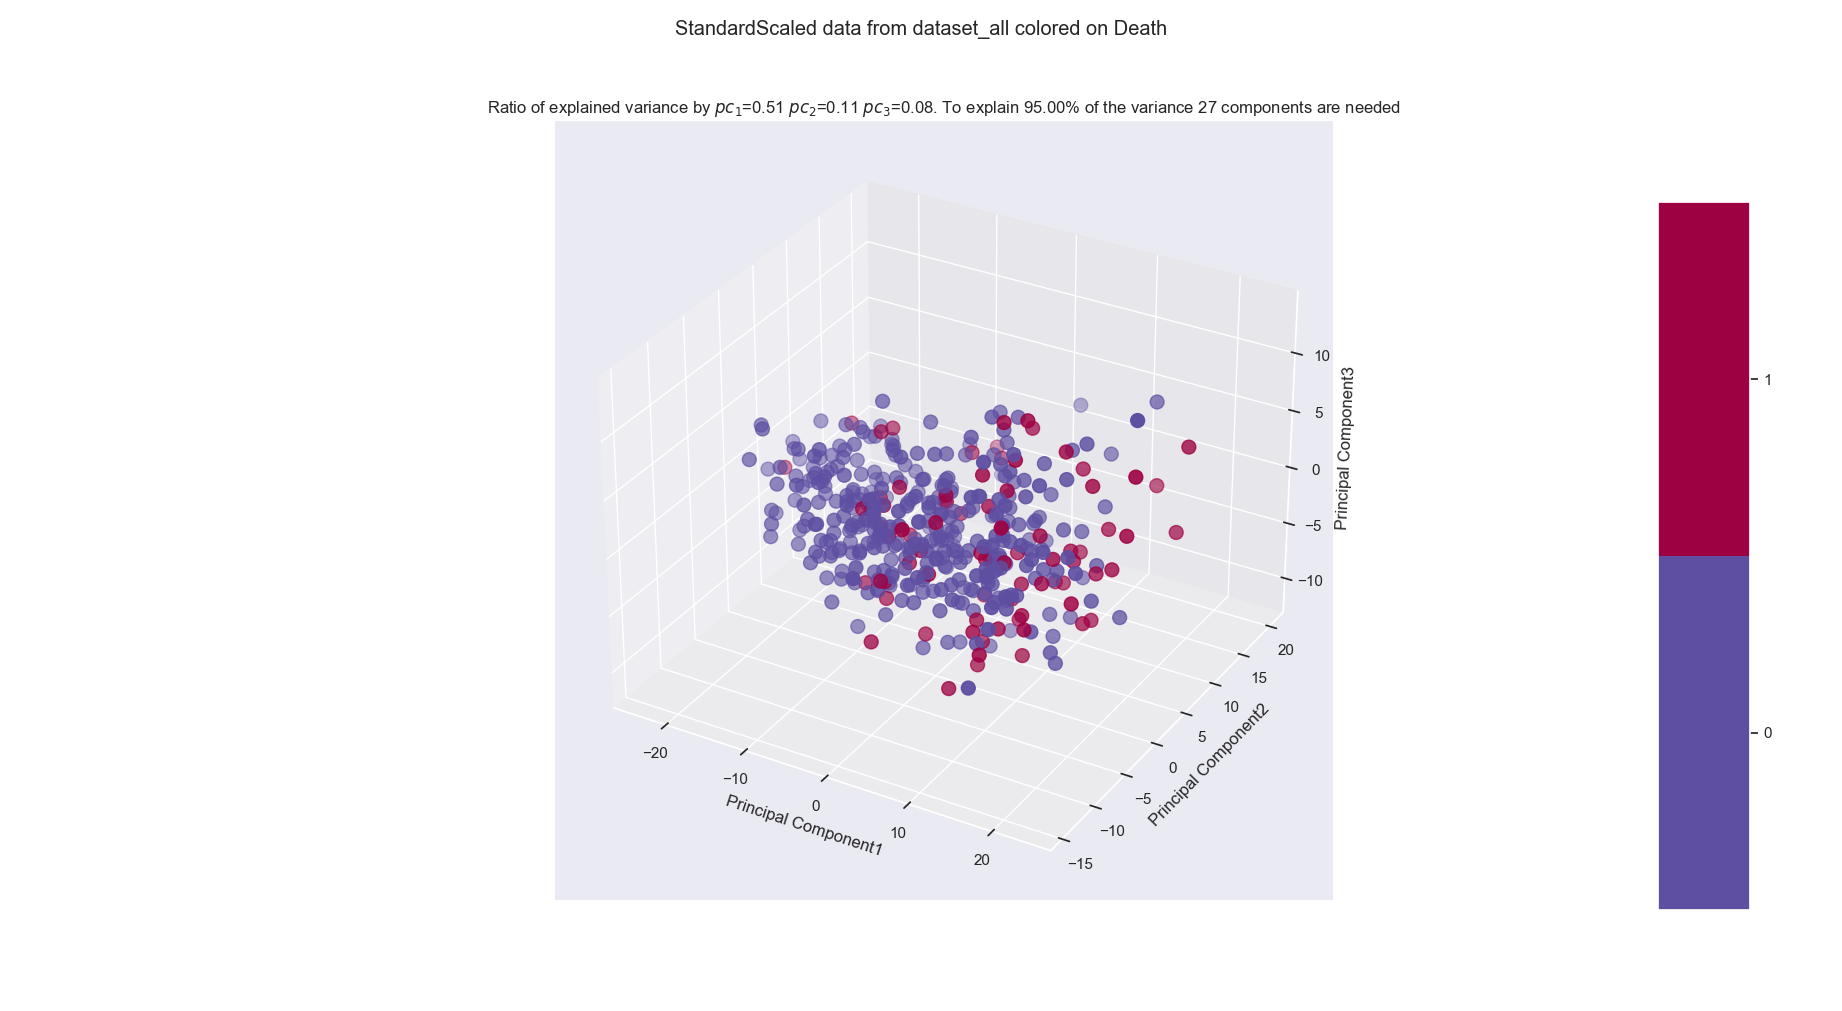
\includegraphics[width=\textwidth]{PCA3_all_Death.png}\label{PCA3_all_death}
  		\caption{3D PCA of whole dataset, colored with death label}
\end{figure}

\begin{figure}[h!]
  		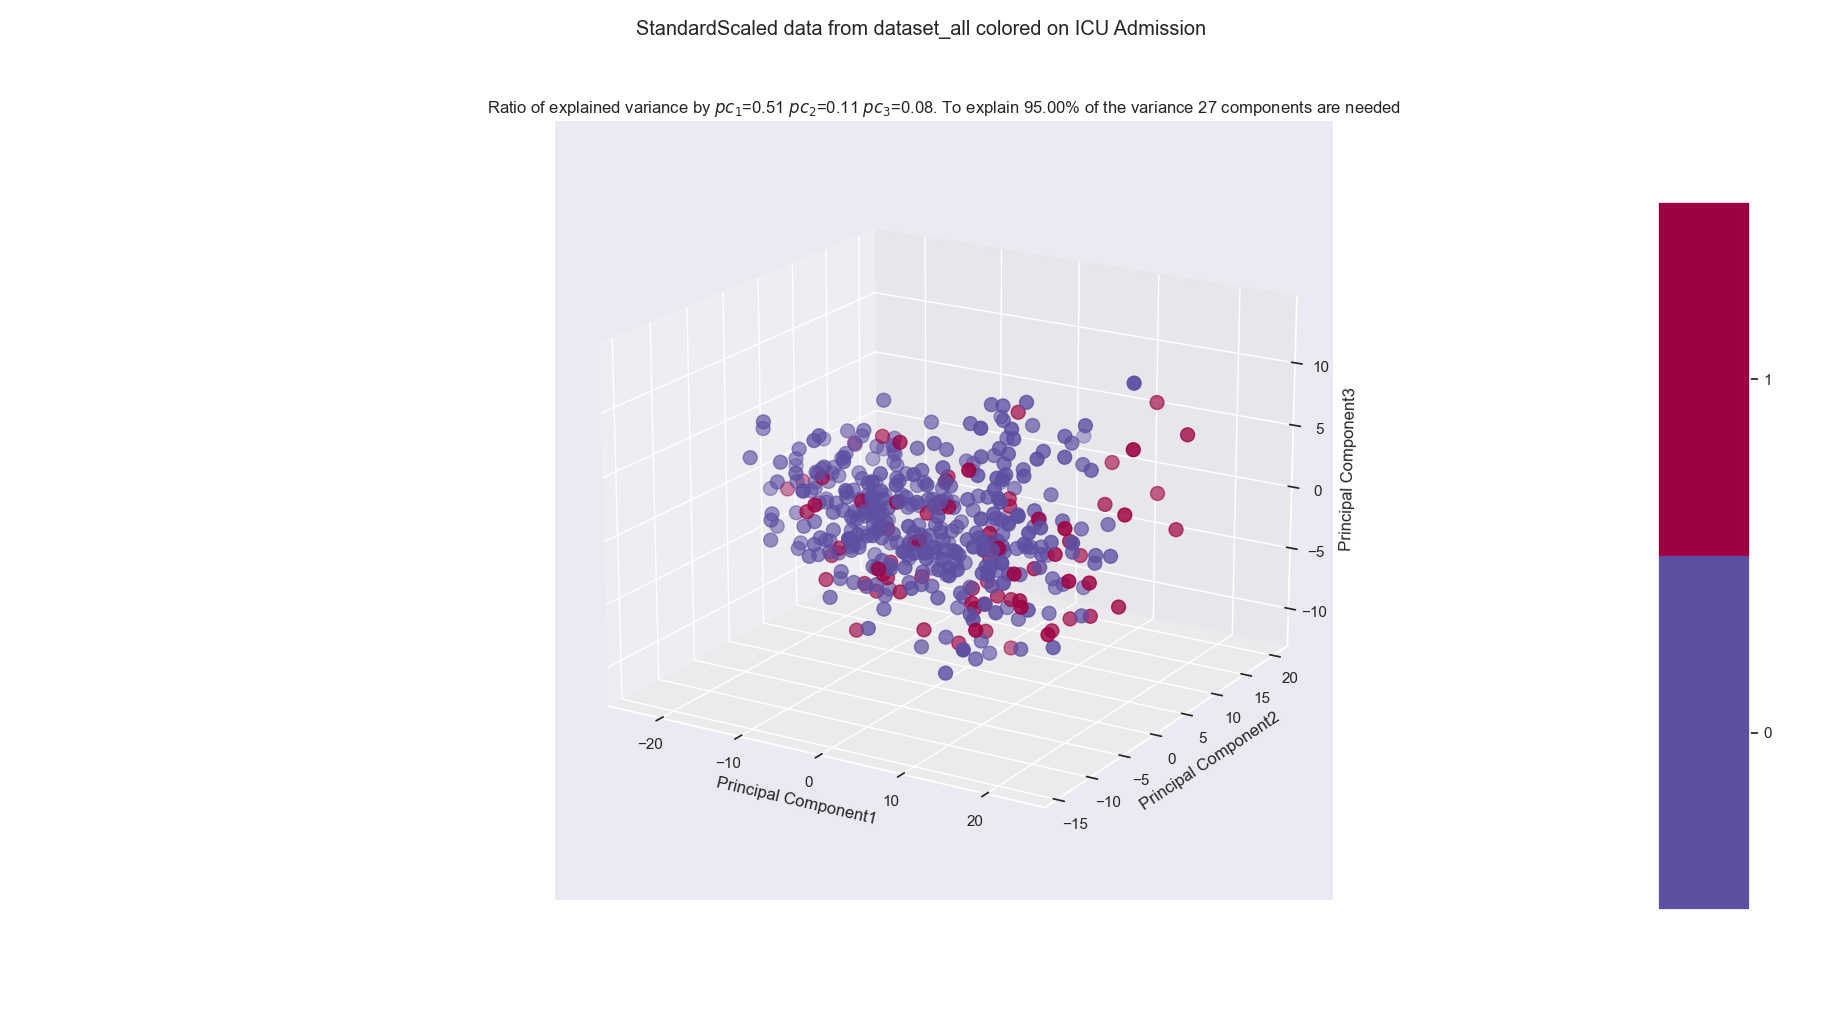
\includegraphics[width=\textwidth]{PCA3_all_ICU.png}\label{PCA3_all_ICU}
  		\caption{3D PCA of whole dataset, colored with ICU Admission label}
\end{figure}

In all cases it seems like introducing the radiomic features causes the loss of the polarization structure that could be seen in the PCA on the clinical dataset alone in fig\ref{fig:PCA2_death}.
 
\begin{figure}[h!]
  		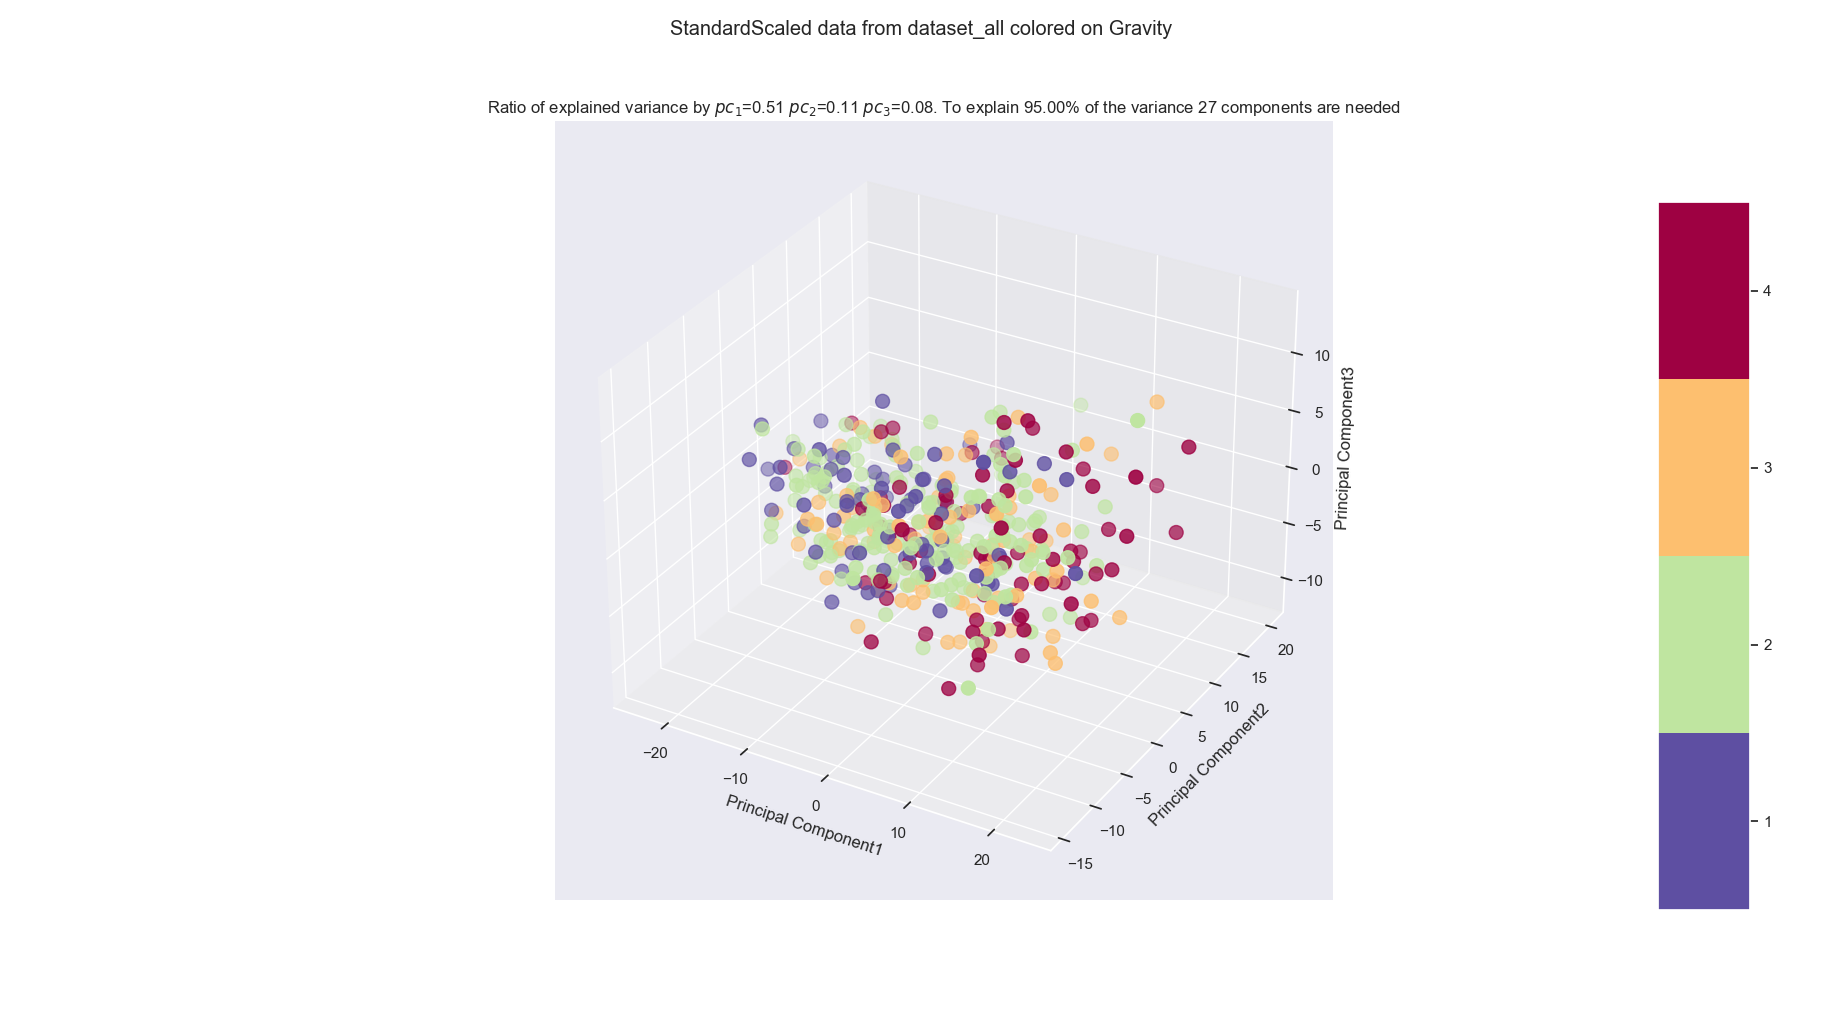
\includegraphics[width=\textwidth]{PCA3_all_Gravity.png}\label{PCA3_all_gravity}
          \caption{Comparison between various colour labels of the top 3 principal components for the entire dataset. Note that to explain 95$\%$ of the variance 27 components would be needed}
\end{figure}

Since there are no visible clusters proceeding with cluster analysis would mean incurring in the risk of finding non meaningful results so it seemed appropriate to try other dimensionality reduction techniques.

\subsection{Exploring data structure with UMAP}
The next technique tried was unsupervised Umap. Following the conclusions derived from fig:\ref{fig:hyperparam_umap} the number of neighbours was set to 10 and the minimum distance was set to 0.
Once again the comparison were made between clinical and radiomic dataset as well as different possible labellings. 
Starting from the clinical dataset, without reporting all labels used, it's clear to see that the dataset seems to indicate very local well separated structures which don't seem correlated to gravity outcome

\begin{figure}[htbp]
  		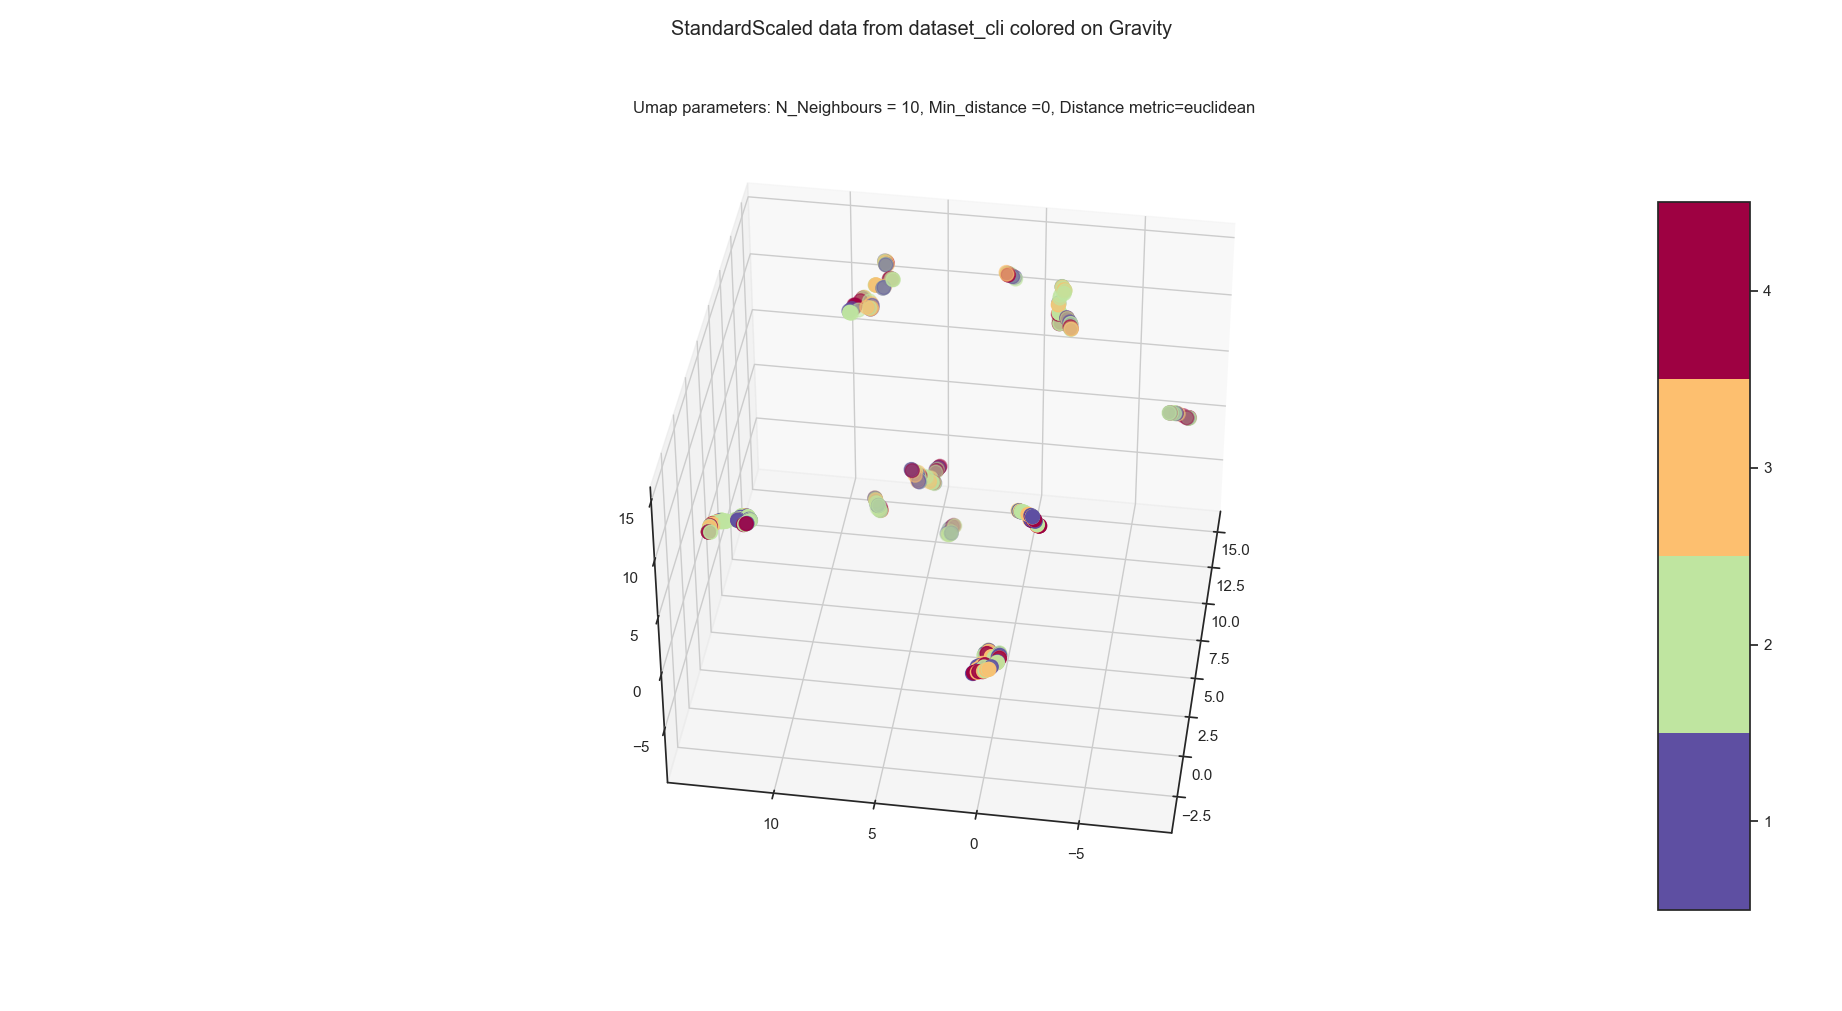
\includegraphics[width=\textwidth]{umap3_cli_Gravity.png}\label{umap3_cli_gravity}
          \caption{3D umap of clinical dataset, colored based on gravity}
\end{figure}

There are 9 well defined groups which don't seem to be correlated to any of the available labels. 
The dimension of these group is also very prohibitive if thinking of further analyses since groups of 35-50 people in a dataset with 15$\%$ mortality rate would mostly be very unbalanced if they were to be used for classification.
However if the introduction of radiomic features were to unite some of these groups then this embedding could be meaningfully used for analysis. 
Looking at the 3D embedding for the whole dataset, the results are:

\begin{figure}[htbp]
  		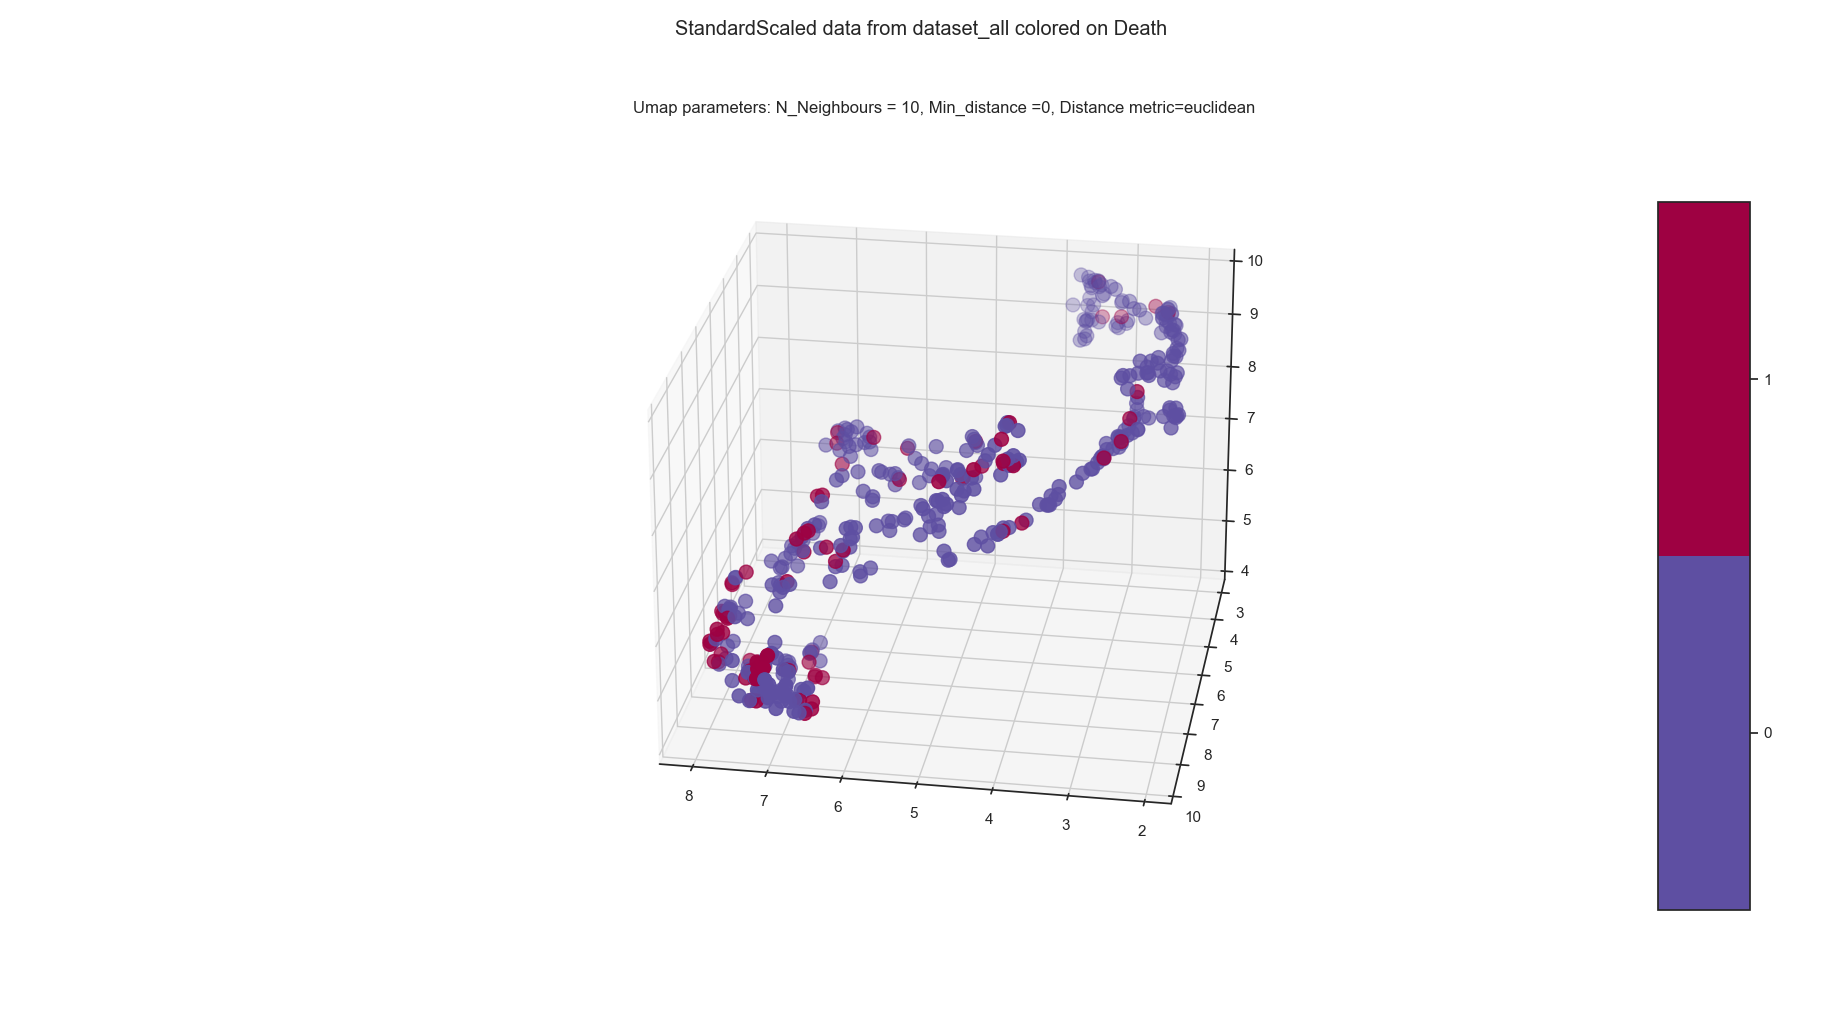
\includegraphics[width=\textwidth]{umap3_all_death.png}\label{umap3_all_death}
          \caption{3D umap of whole dataset, colored based on death}
\end{figure}

\begin{figure}[htbp]
  		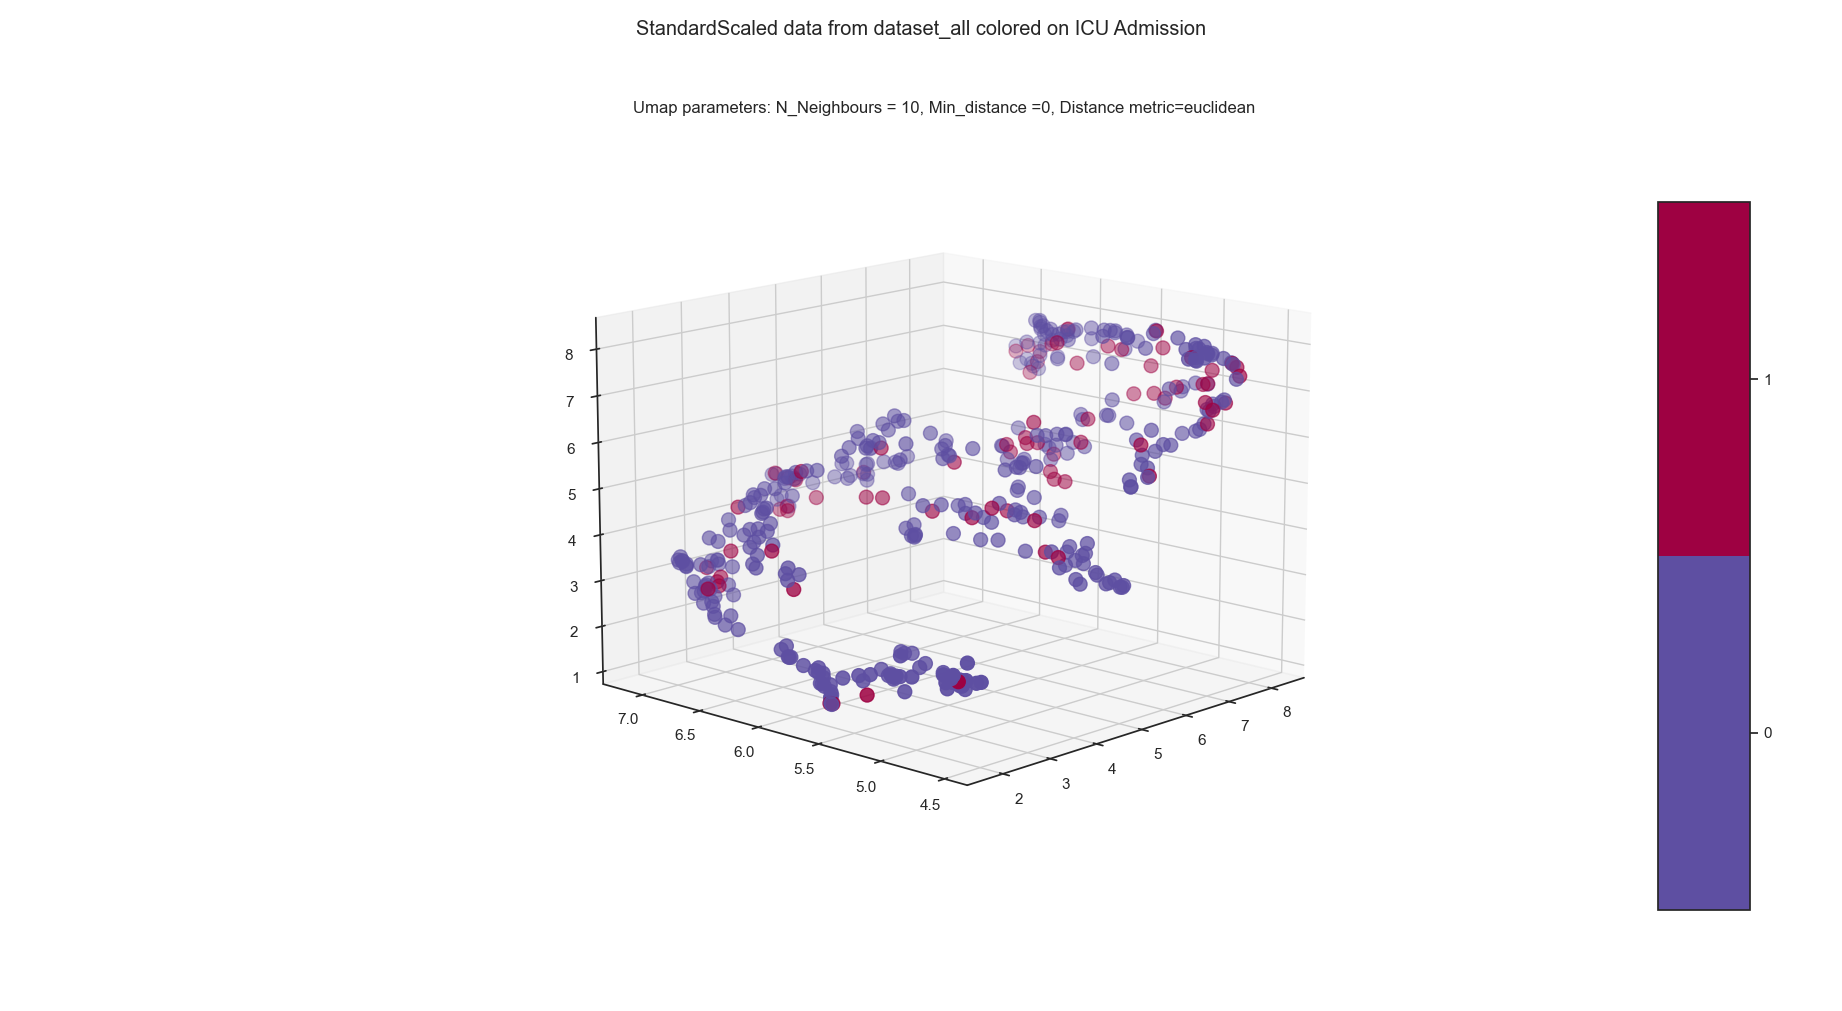
\includegraphics[width=\textwidth]{umap3_all_ICU.png}\label{umap3_all_ICU}
          \caption{3D umap of whole dataset, colored based on ICU admission}
\end{figure}

\begin{figure}[htbp]
  		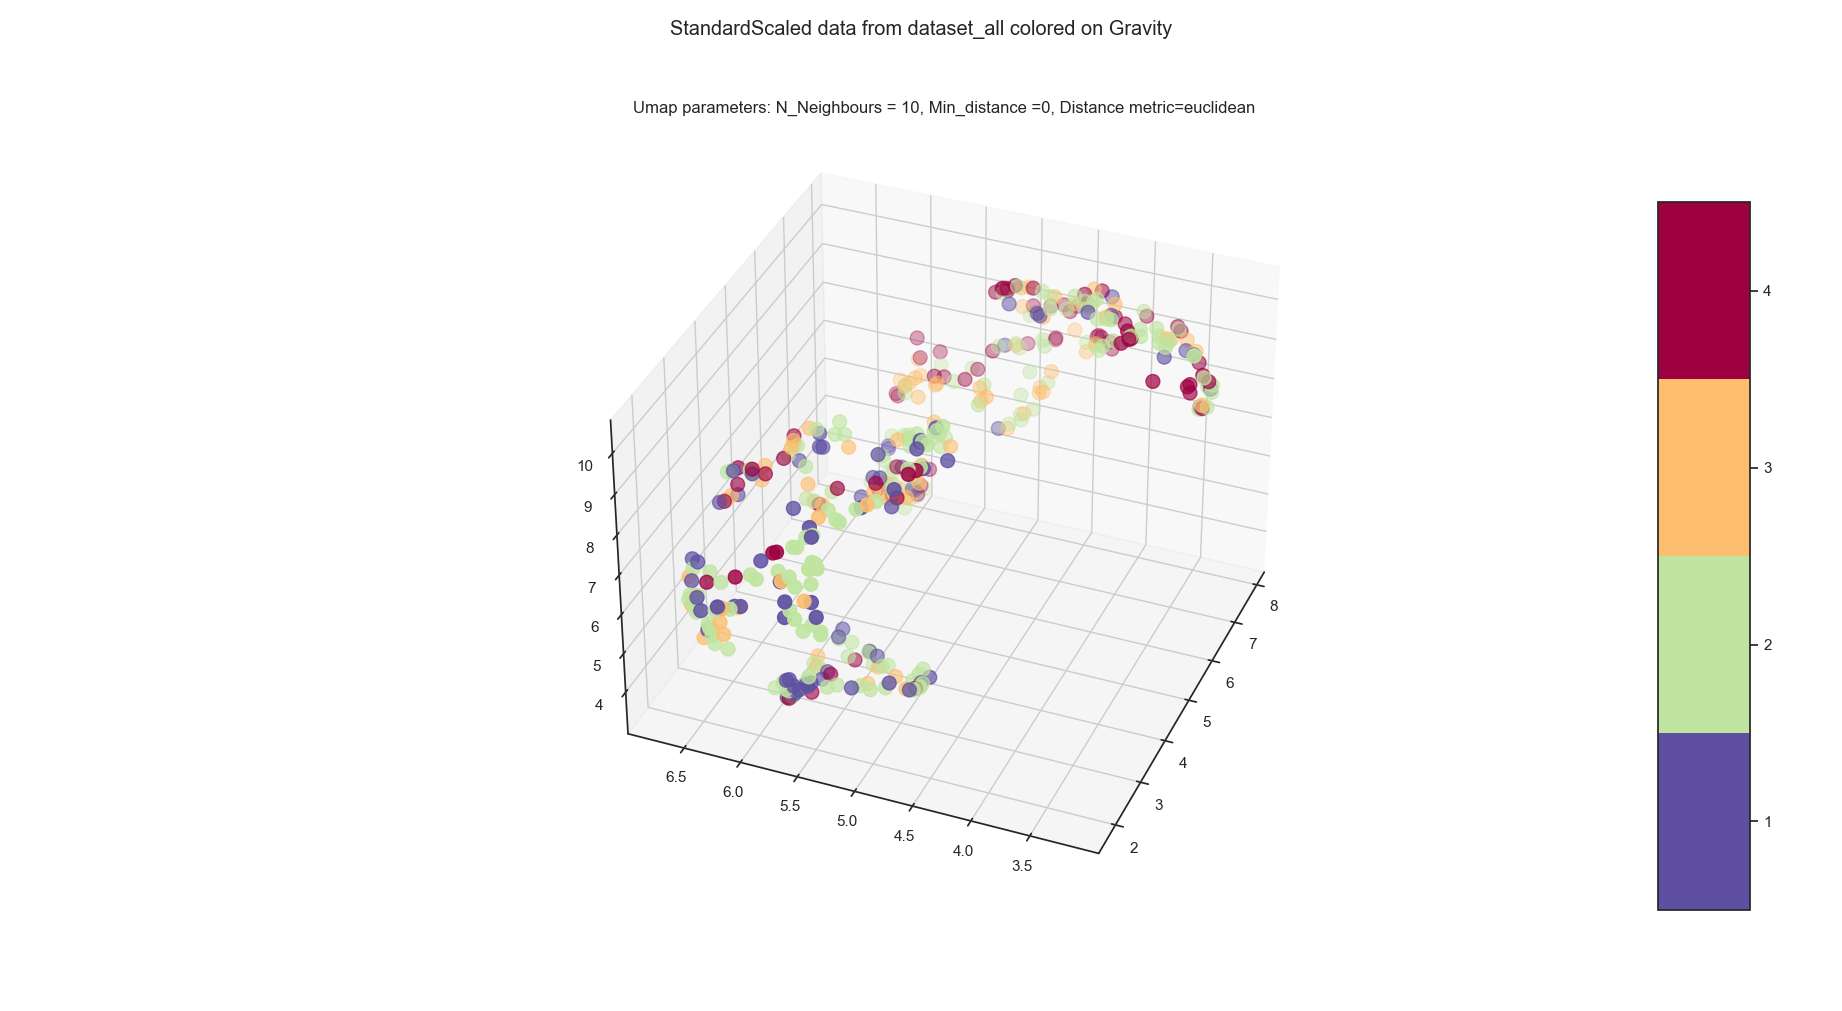
\includegraphics[width=\textwidth]{umap3_all_Gravity.png}\label{umap3_all_Gravity}
          \caption{3D umap of whole dataset, colored based on gravity}
\end{figure}

Once again the introduction of the radiomic feature seems to be a confounding factor in the seemingly clear-cut order present in the clinical dataset alone.
There seems to be a well connected structure, which makes sense because umap sets out with the objective of preserving said structure.
However since the variables of interest as label are Death, ICU admission or some kind of combination of them with hospital permanence there seems to be no visual correlation between structure and label.
As such the next dimensionality reduction was tried to see if it yielded better results.
 
\subsection{Predicting clinical outcome using PLS-DA}
Moving on from unsupervised methods to a supervised one, PLS-DA was used giving as label both death and ICU using both whole dataset, and singularly radiomic or clinical features. 
Starting from the clinical features alone, predicting on death Figure~\ref{PLSDA-Clinical} can be obtained.

\begin{figure*}[htbp]
  		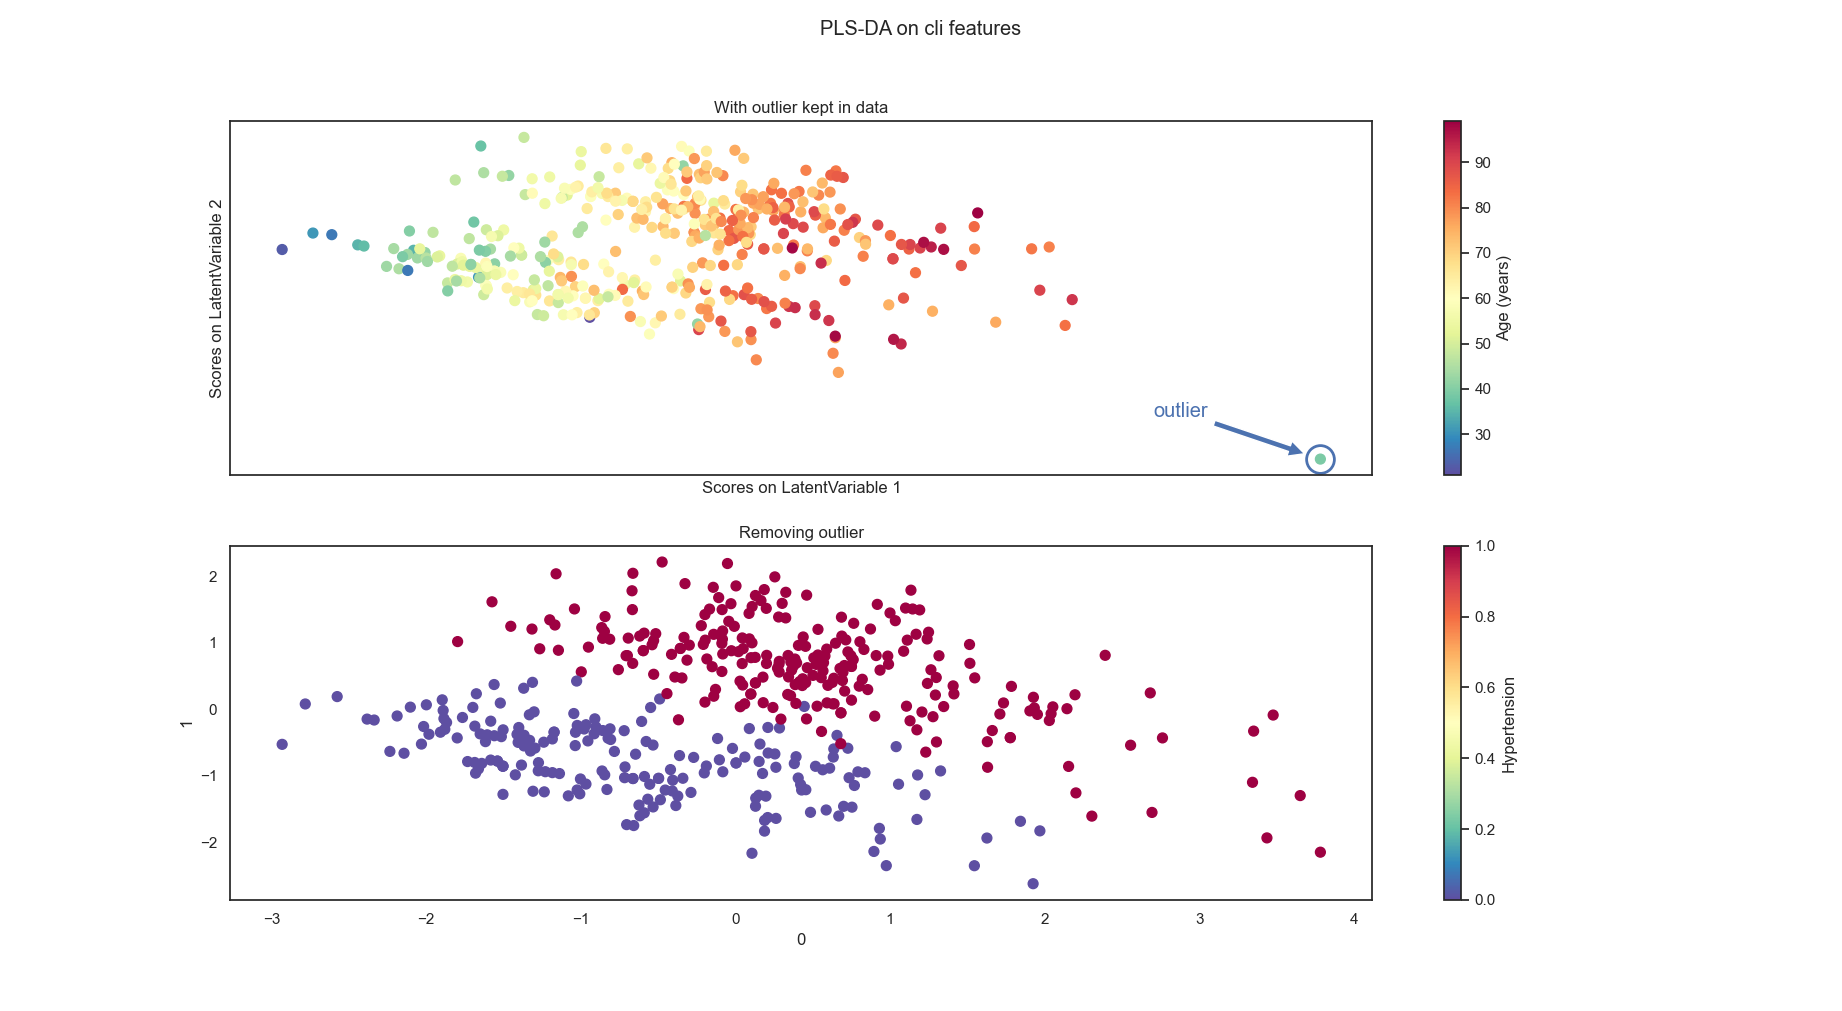
\includegraphics[width=1\textwidth]{Clinical_dataset.png}
          \caption{PLS-DA predicting on death coloured with age and hypertension\label{PLSDA-Clinical}}
\end{figure*}

In Figure~\ref{PLSDA-Clinical} there are a few things to note. 
The first is the presence, in the top plot, of an outlier which, since PLS-DA is based on minimization of least squares, can ruin a lot the performance of the procedure. 
For this reason in the second plot the outlier was removed and the algorithm was run again on the cleaned data.
The second thing to notice is the coloring used which, in the first plot, was used to highlight that along the one of the two latent variables the data is roughly distributed depending on age while, in the second plot, was used to highlight that the algorithm is able to perfectly separate the subjects with hypertension from those without it.
However, by looking at the same embedding labelled with death and ICU admission fig \ref{PLSDA-Clinical-death} can be obtained

\begin{figure}[htbp]
  		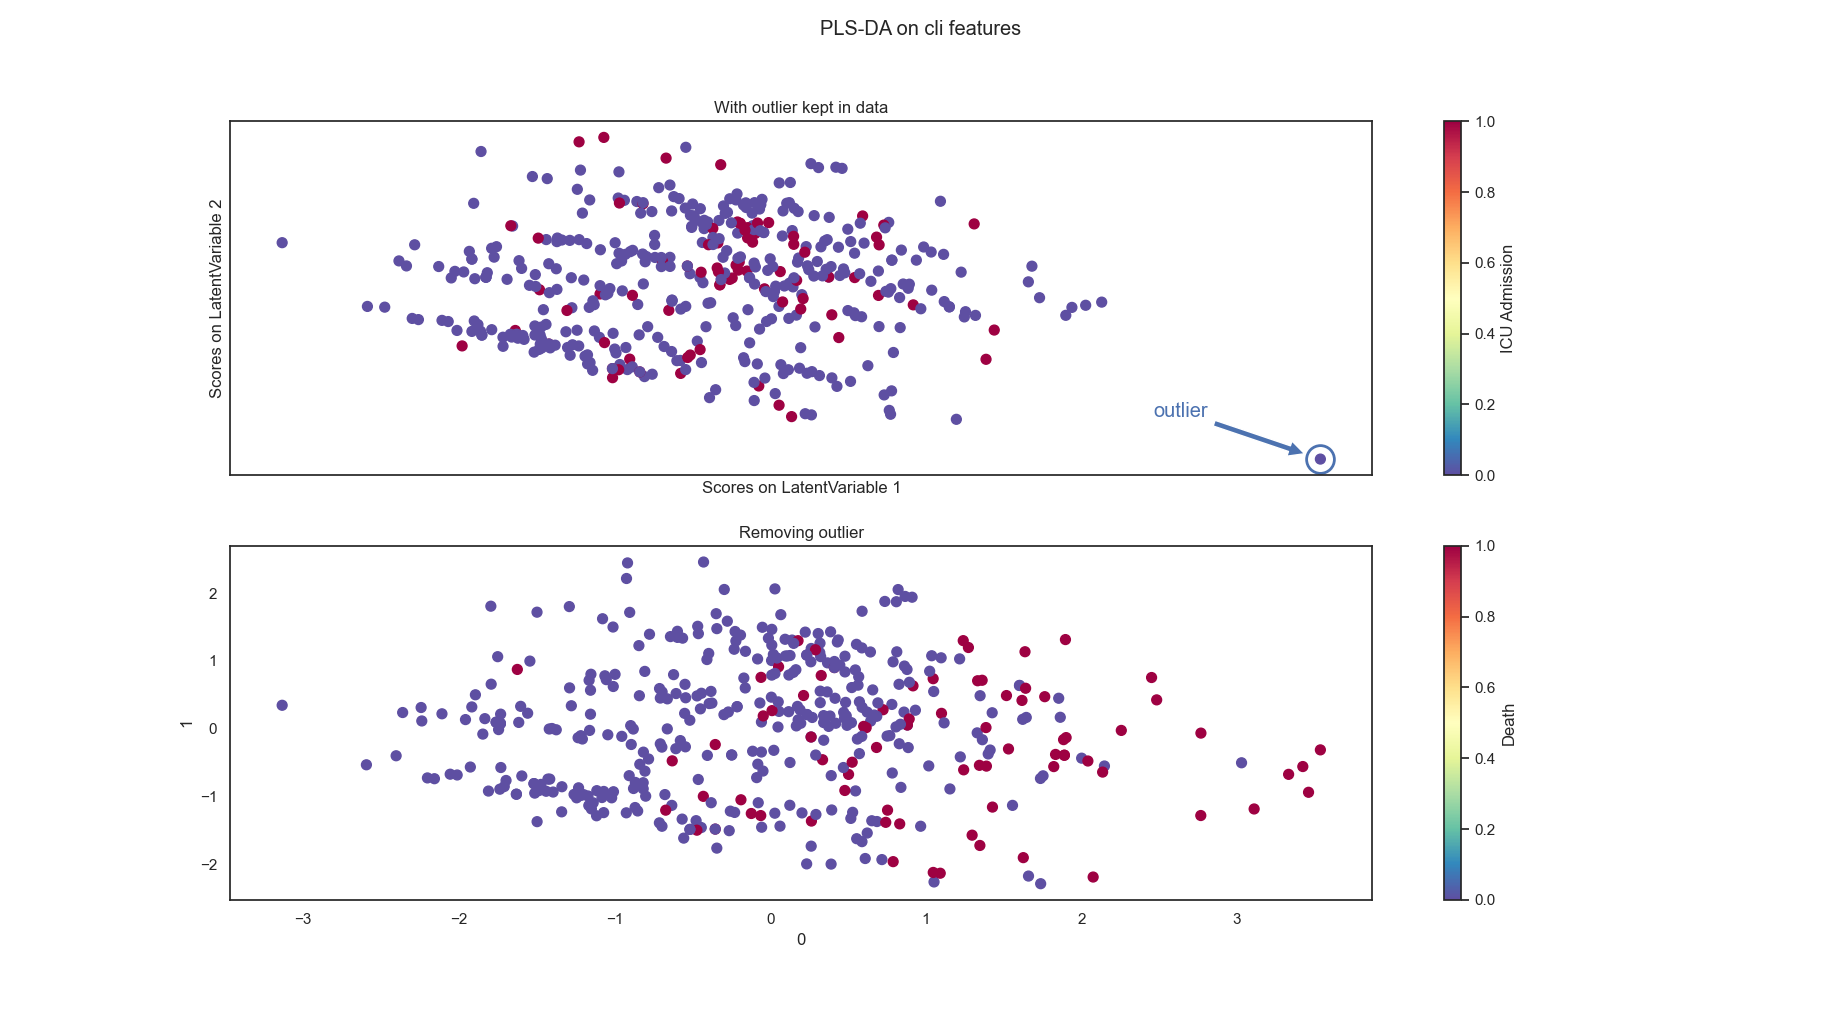
\includegraphics[width=\textwidth]{PLSDA_cli_death.png}
          \caption{PLS-DA predicting on death coloured with death(bottom) and ICU Admission(top)\label{PLSDA-Clinical-death}}
\end{figure}

It's clear to see that, when predicting on death, the PLS-DA algorithm doesn't find any behaviour relevant for ICU admission.
It's also clear that there is at least a pattern of points labelled as dead being towards the right of the image, this can be easily explained by looking at how the ages are distributed in the first plot of fig: \ref{PLSDA-Clinical}. 
From this it's possible to deduce that older individuals tend to die more and that hypertension does not seem to be relevant when considering death as a clinical outcome.
If necessary the PLS-DA algorithm allows also to see the weights given to the features in predicting the label. At least for the clinical dataset, which has a reasonable number of features, it's interesting to report it ordering the coefficients by descending absolute value: 

\begin{table}
\caption{PLS-DA feature weights in prediction on death using clinical features}
\centering
	\begin{tabular}{|l|r|}
	\hline
	Feature Name &         Importance \\
	\hline
	 Respiratory Rate &  0.120206 \\
	 Age (years) &  0.116305 \\
	 Obesity &  0.004293 \\
	 Hypertension & -0.004626 \\
	 History of smoking & -0.012314 \\
	 Febbre & -0.045431 \\
	 Sex\_bin & -0.054947 \\
	\hline
	\end{tabular}
\end{table}

Doing the exact same procedure on the whole dataset, which means by including the radiomic features, Figure~\ref{fig:whole_dataset} can be obtained.

\begin{figure}[htbp]
  		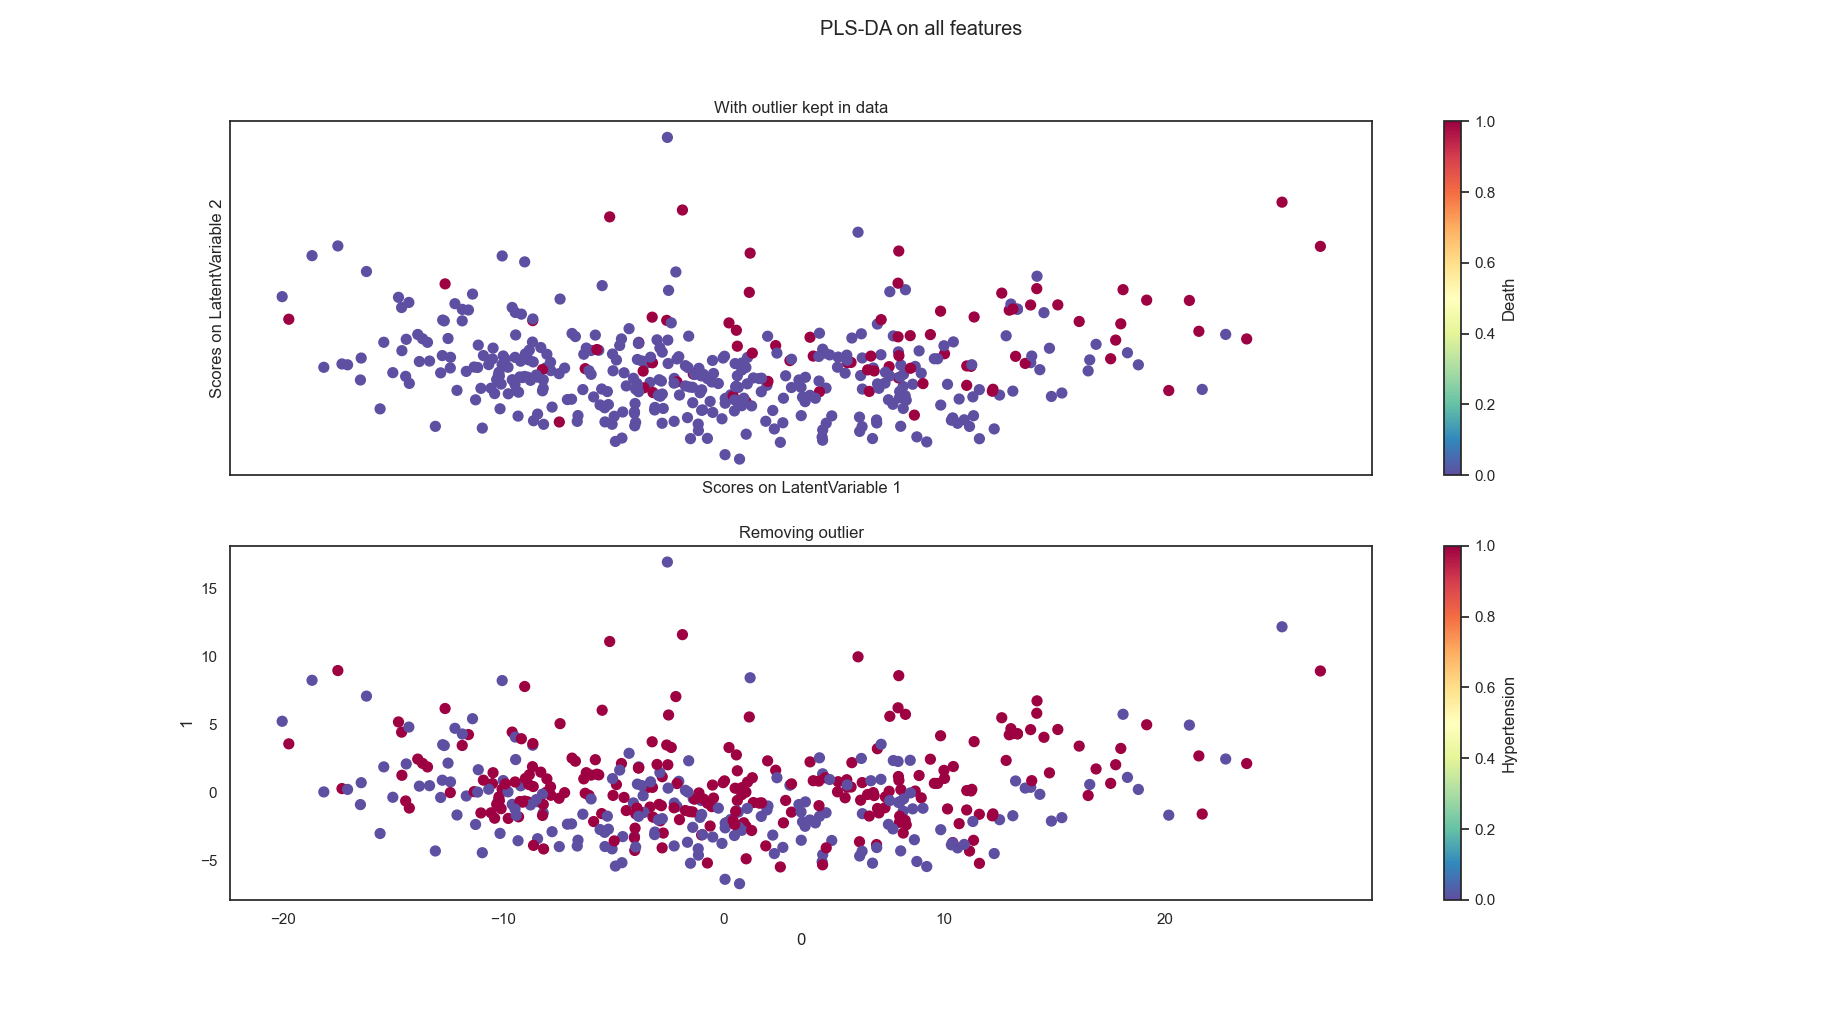
\includegraphics[width=\textwidth]{Whole_dataset.png}
          \caption{PLS-DA predicting on death coloured with death(top) and hypertension(bottom) on whole dataset\label{fig:whole_dataset}}
\end{figure}



\begin{figure*}[htbp]
  		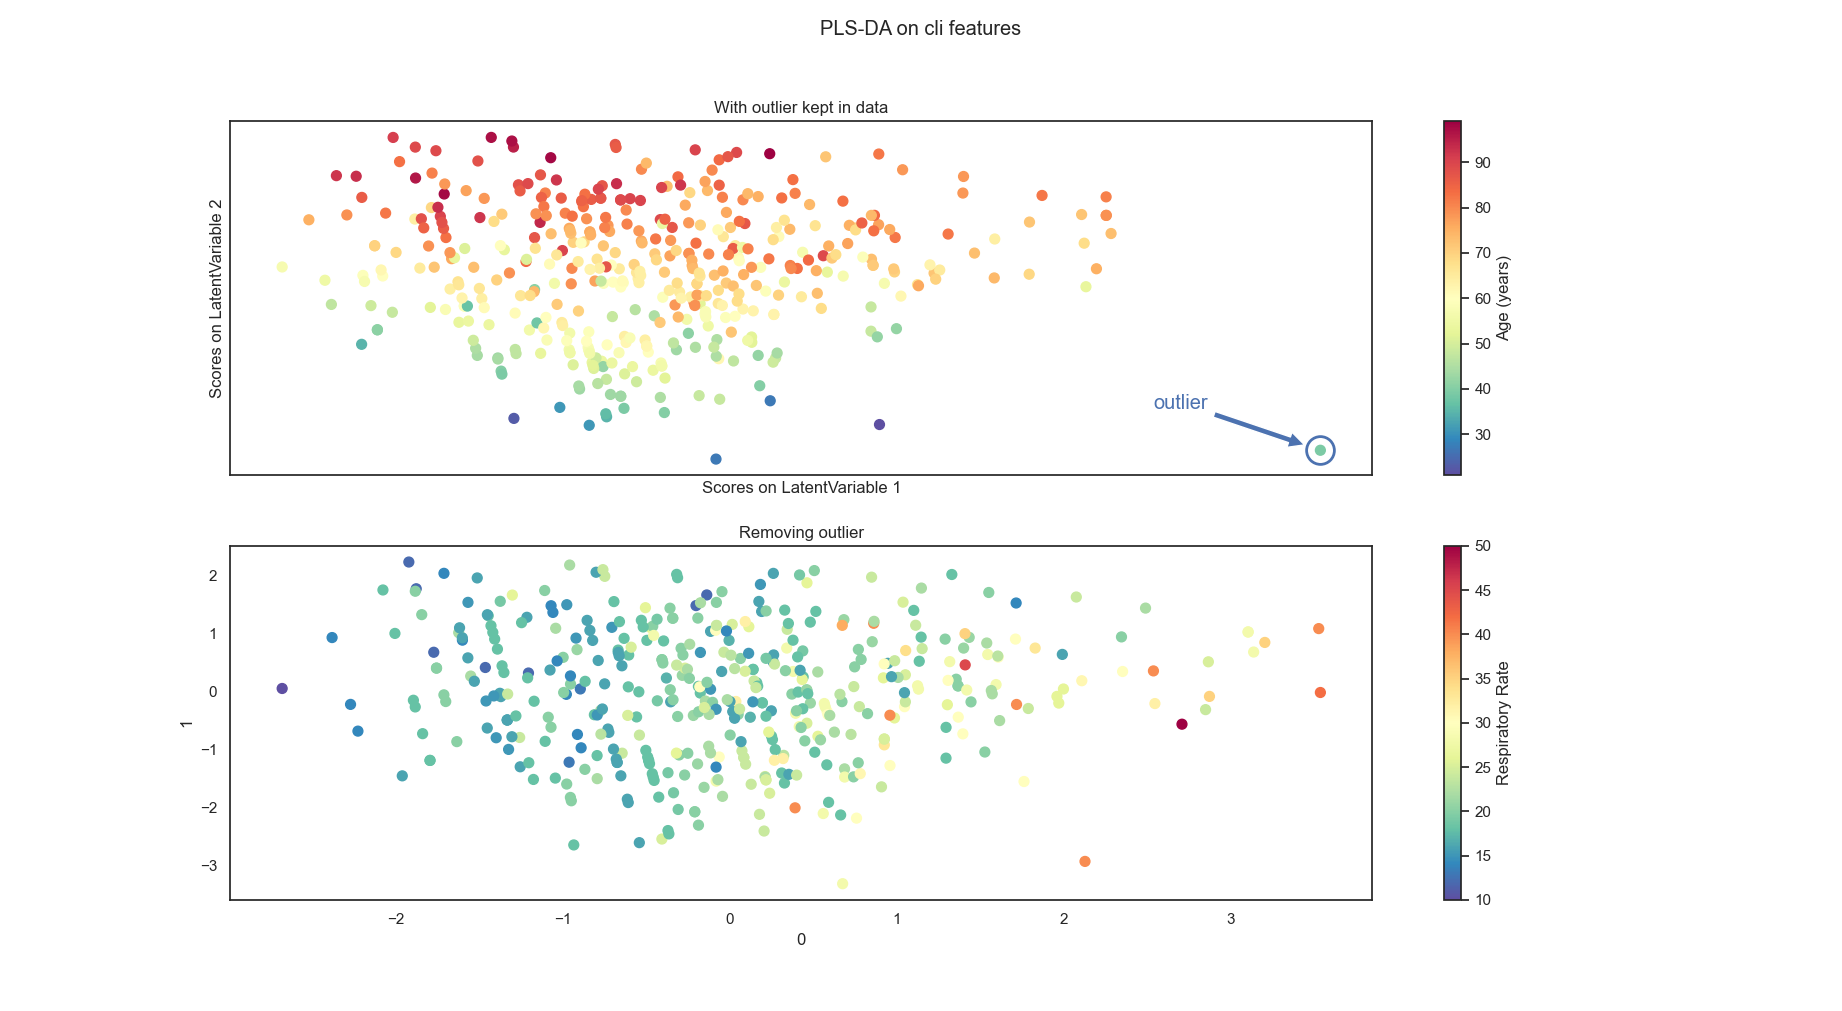
\includegraphics[width=1\textwidth]{PLSDA_cli_ICU_LV.png}
          \caption{PLS-DA predicting on death coloured with Age and respiratory rate on clinical features\label{fig:PLSDA-ICU-LV}}
\end{figure*}

Once again adding the radiomic features has evidently introduced noise in the system, which no longer displays any kind of behaviour, pattern nor separation.
Doing the same analysis but using ICU Admission as a label Figure~\ref{fig:PLSDA-ICU-LV} can be obtained. 

Now the colors have been chosen to highlight that respiratory rate and age have the main role in determining the latent variables. However, in this case, there doesn't appear to be a clear cut distinction as it happened before with hypertension.
Looking at how the points scatter by coloring them according to the two interesting clinical labels the following figure can be obtained:

\begin{figure}[H]
  		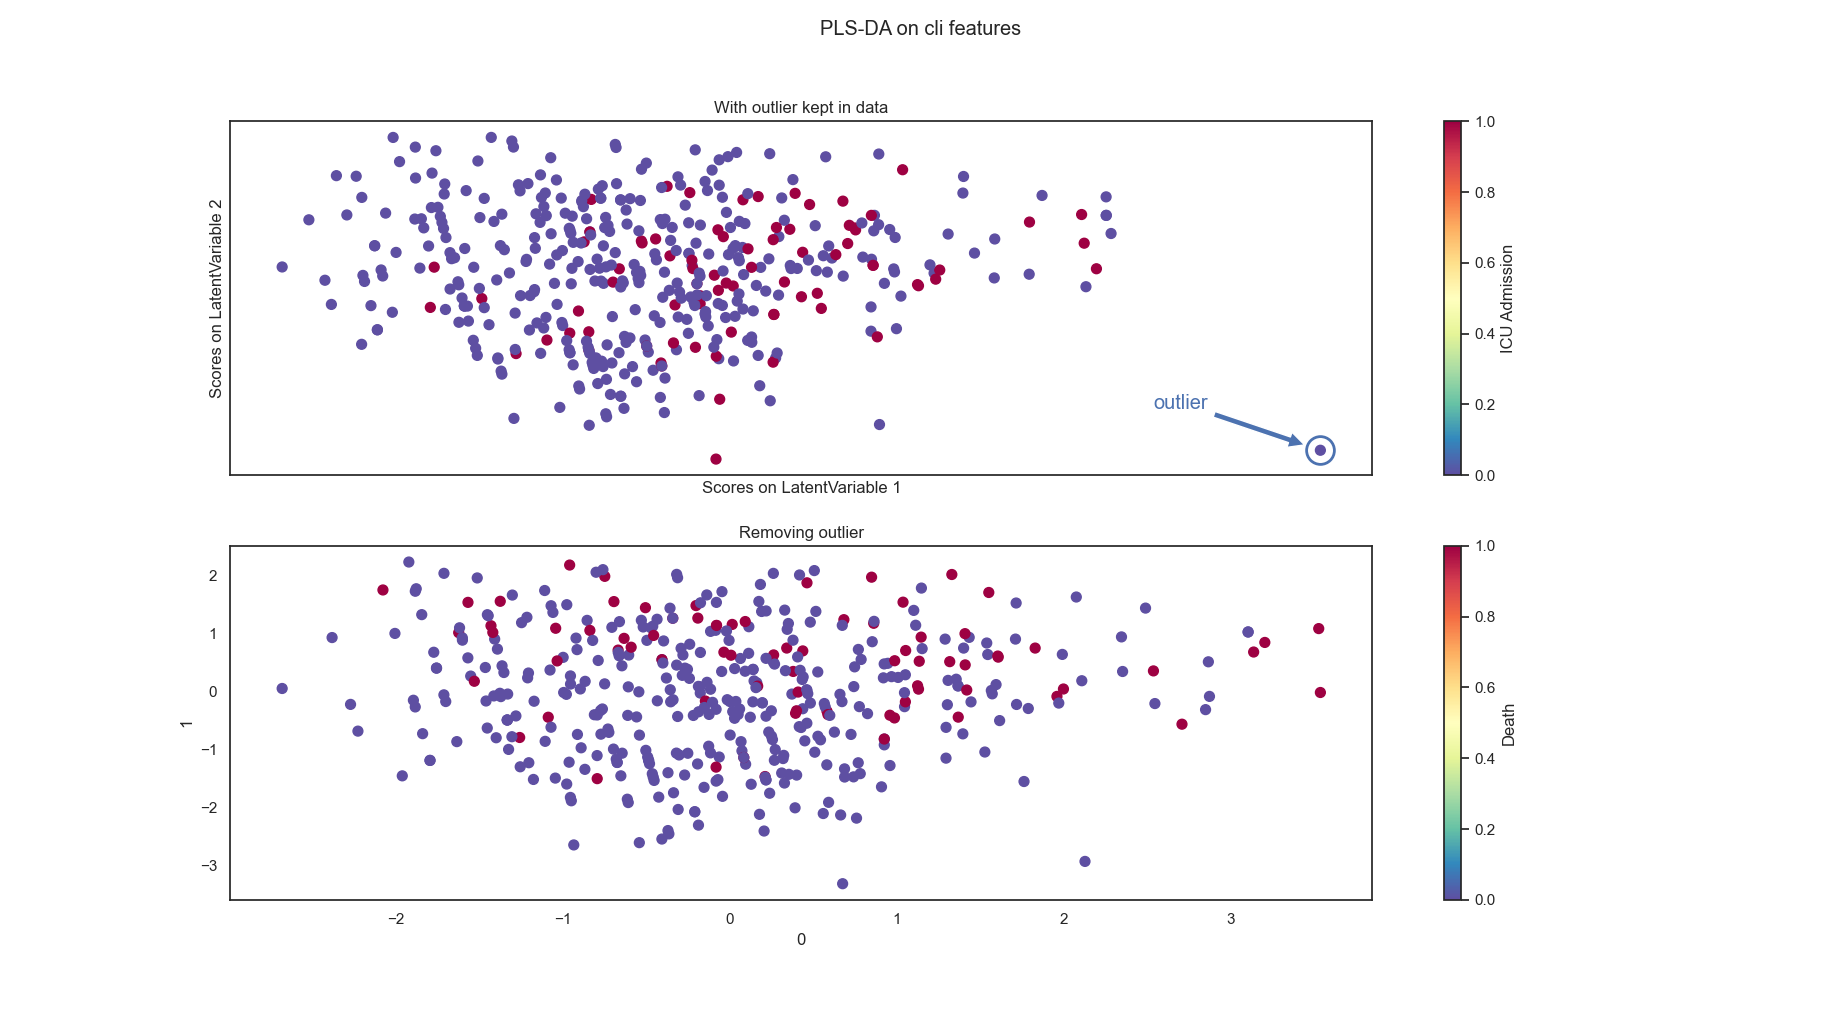
\includegraphics[width=\textwidth]{PLSDA_cli_ICU.png}
          \caption{PLS-DA predicting on death(bottom) coloured with death and ICU admission(top) on clinical features\label{fig:PLSDA-ICU}}
\end{figure}

Finally, introducing the radiomic features in the analysis the usual effect of reducing separation can be seen in the figure below:

\begin{figure}[H]
  		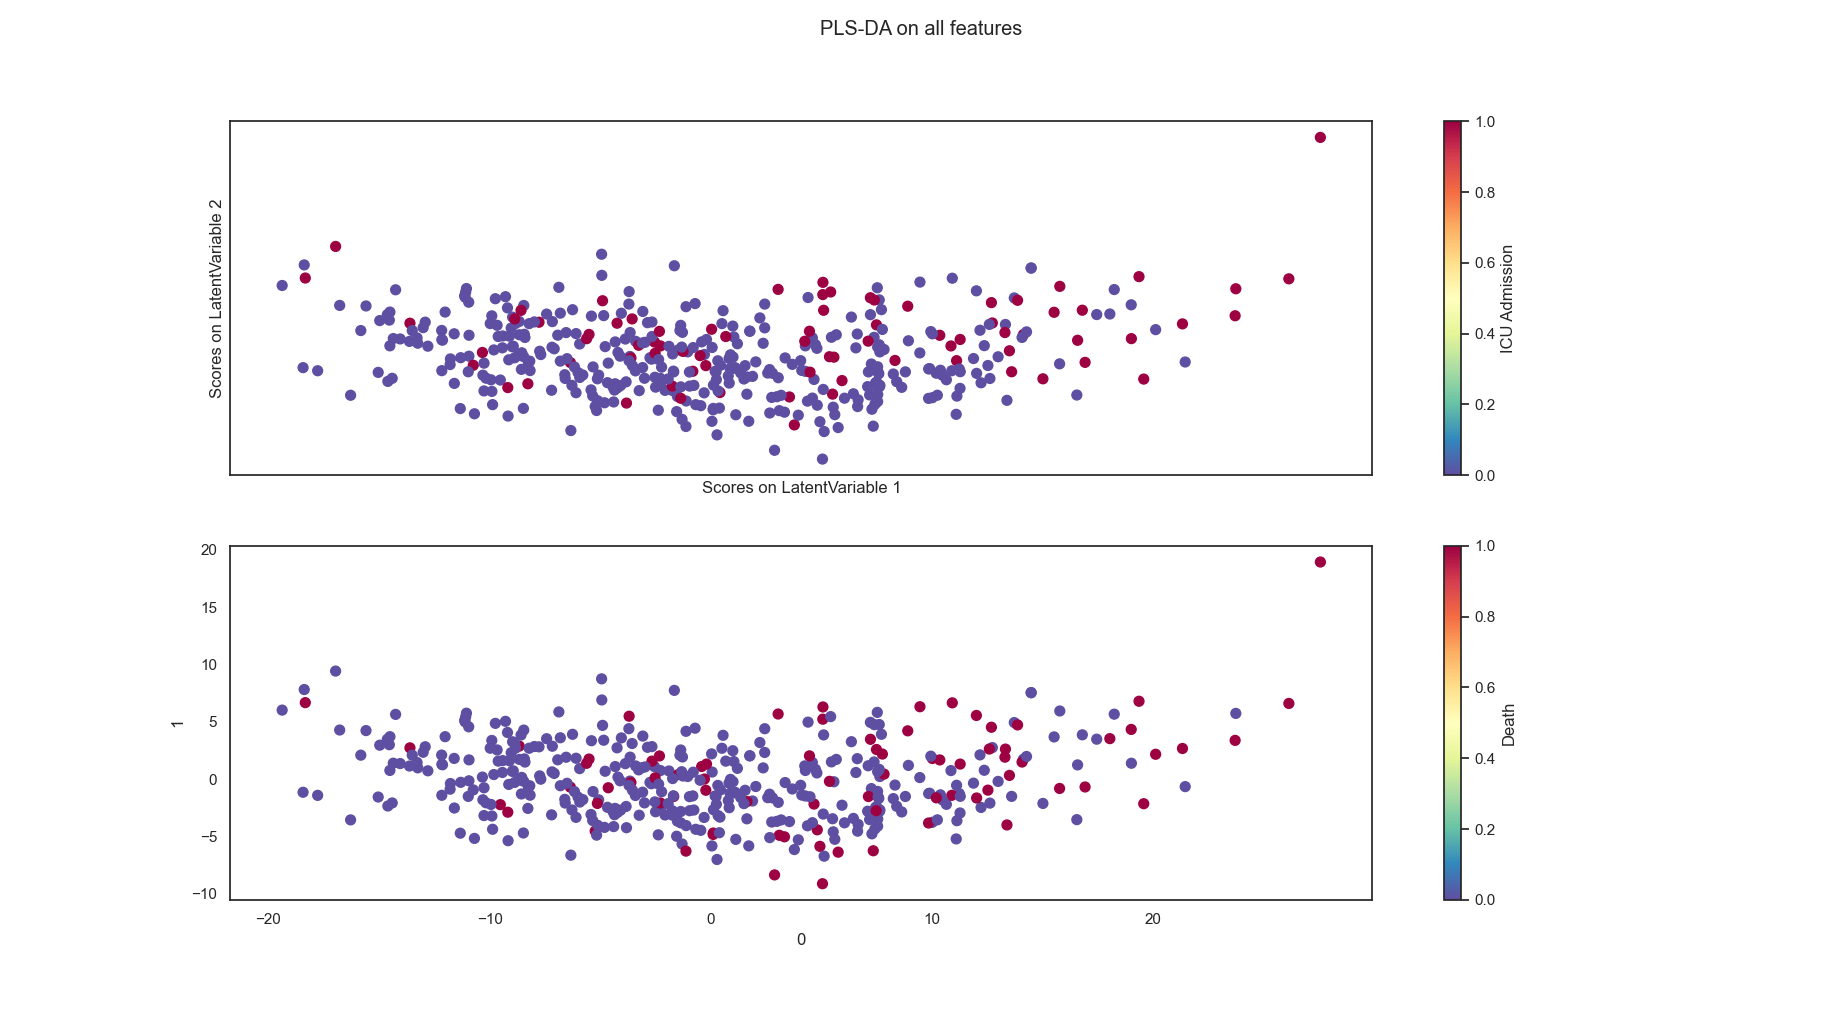
\includegraphics[width=\textwidth]{PLSDA_all_ICU.png}
          \caption{PLS-DA predicting on death coloured with death(bottom) and ICU admission(top) on all available features\label{fig:PLSDA-ICU-all}}
\end{figure}
 
In conclusion various dimensionality reduction techniques have been used while looking for meaningful groups in the patient cohort, trying to understand if successive steps in the data analysis required specific care. Starting from a dataset with 7 clinical features, 179 radiomic features and 8 radiological features using PCA, Umap and PLS-DA the data was reduced to the top three, or two, most informative combinations of features found by each method.

Using PCA it became evident that there were no peculiar combination of features that explained most of the variance, and that this held for all of the feature categories and their combinations. 

Using UMAP it became clear that the data has a peculiar distribution and relationship in the whole feature space, however it seems that this structure is not correlated with the clinical outcomes of interest, main of which being the labels for ICU Admission and Death. 

Finally using PLS-DA it was found that there is an obvious correlation between age and death, which is not surprising. It was also found that the algorithm, while trying to predict death, perfectly separates patients affected by hypertension from those without it. This is not  a result because hypertension is one of the variables available in the clinical dataset, yet it might indicate that some combination of the other features can be expected to correlate with this single one. While using either death and ICU Admission as labels no clear separation of data can be found.

The most relevant concept to note, however, is that introducing radiomic features does not improve the separation in the data.
This is relevant because it can be taken as symptom of minor imperfections in the radiomic features.

More specifically since the segmentation was based on thresholding and region growing methods, this can indicate that in the case of COVID-19 damage, which may heavily alter the gray levels in the lung, these methods have room for improvement.